In the literature, a multitude of meta-heuristic algorithms have emerged over
the years, exploring various ideas to guide the search
process~\cite{osman1996metaheuristics}. These encompass strategies that narrow
the search space to promising regions, enhance solutions in a greedy manner, or
utilize randomized and probabilistic techniques, some of which draw inspiration
from natural phenomena like collective behavior, natural selection, and physical
processes of materials.

However, the majority of state-of-the-art meta-heuristic algorithms can be
described by a few distinctive traits~\cite{blum2003metaheuristics} such as:

\begin{description}
  \item[\textbf{Search Strategy.}] This refers to the method used to find a
    solution.~It can be one of three main types: constructive, local, or a
    \emph{composite} approach that combines both strategies.

  \item[\textbf{Memoization.}] This concept involves maintaining a record or
    archive of previously explored solutions.~This record helps in identifying
    solutions that may be revisited or disregarded in subsequent stages of the
    optimization process.

  \item[\textbf{State Size.}] This pertains to the number of solutions being
    evolved during the construction phase.~In~\emph{population methods}, multiple
    solutions are worked with at each iteration, while in~\emph{trajectory methods} (single-state),
    only a single solution is improved at a time.
\end{description}

In this section, we will offer a brief overview of select state-of-the-art
\acrshort{meta-heuristic} algorithms, which encapsulate all the above properties
and will be utilized and implemented in the context of this work.

\subsection{Beam Search}
\label{subsec:beam-search}

\acrfull{beam-search}~\cite{ow1988filtered,outeiro2021application} is a
\acrshort{constructive-search} population~\acrfull{meta-heuristic} inspired by
the~\emph{breadth-first search} algorithm~\cite{papadimitriou1998combinatorial}.
However, it deviates from the conventional practice of expanding all solutions
in the search tree during each iteration. Instead, this technique maintains a
fixed-size archive of previous solutions, which are expanded at each
step~(\textit{beam}). Subsequently, the expanded solutions undergo filtering,
and only the best solutions, determined based on heuristic information or bound
values, are retained within the archive. These selected solutions act as the
starting points for the next iteration. It is important to acknowledge that the
size of this archive, and consequently the number of solutions filtered at each
step, is dictated by a parameter referred to as the~\emph{beam width}.

The construction process of~\acrshort{beam-search} terminates either when there
are no more candidate solutions to expand or when other predetermined stopping
criteria are satisfied. For illustration purposes, the pseudocode for
\acrshort{beam-search} is presented in \Cref{algorithm:beam-search}.
In this context, the notation $\argmax_{w}$ is employed to introduce the concept
of selecting the top $w$ elements from a given set.

\begin{algorithm}[h]
  \begin{frame}{Problem}
  This problem entails the setup of scanning pipeline for books.

  \begin{itemize}
    \item There are libraries housing various books. Before any scanning can commence, each
          library needs to register for the scanning process. Once registered, each
          library is allowed to scan a certain number of books daily, until global deadline.
    \item Only one library can undergo the sign-up process at any given time.
    \item Each book, when scanned, contributes a specific score.
  \end{itemize}

\end{frame}

\begin{frame}{Example --- Book Scanning}
  \begin{figure}[h]
    \centering
    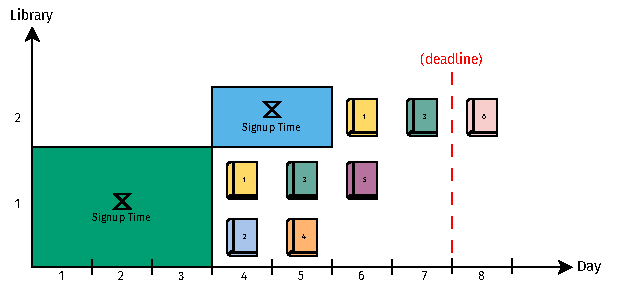
\includegraphics[width=0.8\textwidth,keepaspectratio]{../assets/bs/bs-example-slides.pdf}
    \caption{Book Scanning Example}
  \end{figure}

  \begin{table}[ht]
    \centering
    \begin{tabular}{ccccccc}
      \toprule
      \textbf{Book}  & 1 & 2 & 3 & 4 & 5 & 6 \\ \midrule
      \textbf{Score} & 3 & 1 & 5 & 4 & 7 & 1 \\
      \bottomrule
    \end{tabular}
    \caption{Book Scores}
  \end{table}
\end{frame}

\begin{frame}{Problem Formulation}
  \begin{equation*}
    \begin{aligned}
      \max\ f(x) =\  & \sum_{b = 1}^{\mathcal{B}}{s_{b} \cdot \min\left(\sum_{i = 1}^{\mathcal{I}}{x_{b, \phi_{i}^\mathcal{I}}} , 1\right)}                                                                     \\
      \text{s.t }    & \sum_{b = 1}^{\mathcal{B}}{x_{b, \phi_{i}^\mathcal{I}}} \leq r_{i} \cdot \left(\mathcal{D} - \sum_{k = 1}^{i}{t_{\phi_{k}^\mathcal{I}}} \right) \quad \forall i = 1, \ldots, \mathcal{I} \\
                     & \sum_{i = 1}^{\mathcal{I}}{t_{\phi_{i}^\mathcal{I}}} \leq \mathcal{D}                                                                                                                    \\
    \end{aligned}
  \end{equation*}
  Where,
  \begin{itemize}
    \item $\mathcal{B}$ is the number of books.
    \item $\mathcal{D}$ is the global deadline.
    \item $\mathcal{I}$ and $\phi^\mathcal{I}$ are the number and order of signed-up libraries.
    \item $t_{i}$ and $r_{i}$ are the sign-up time and book scanning rate of library $i$.
    \item $s_{b}$ is the score of book $b$.
    \item $x_{b,i}$ is binary variable indicating if a book, $b$, is assigned (1) or not (0) to library $i$.
  \end{itemize}
\end{frame}


\begin{frame}{Example --- Objective}
  \begin{figure}[h]
    \centering
    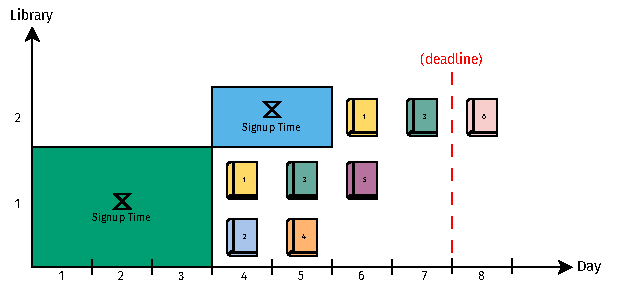
\includegraphics[width=0.8\textwidth,keepaspectratio]{../assets/bs/bs-example-slides.pdf}
  \end{figure}
  \begin{table}
    \begin{tabular}{cc}
      \begin{minipage}{0.5\textwidth}
        \begin{table}[ht]
          \centering
          \begin{tabular}{ccccccc}
            \toprule
            \textbf{Book}  & 1          & 2          & 3          & 4          & 5          & 6 \\ \midrule
            \textbf{Score} & \textbf{3} & \textbf{1} & \textbf{5} & \textbf{4} & \textbf{7} & 1 \\
            \bottomrule
          \end{tabular}
        \end{table}
      \end{minipage}
       &
      \begin{minipage}[b]{0.5\textwidth}
        \centering
        \begin{equation*}
          f(x) = 3 + 1 + 5 + 4 + 7 = 20
        \end{equation*}
      \end{minipage}
    \end{tabular}
    \caption{Book Scores \& Objective Value}
  \end{table}
\end{frame}

\begin{frame}{Modeling --- Problem, Solution and Component}
  The~\alert{problem} is characterized by the set of all libraries available, along with
  their sign-up times, book shipping rate, and list of books that can be shipped,
  the scores for all the books, and the deadline.

  A~\alert{solution} is characterized by a collection of assignments of books
  to libraries and the order in which libraries are scanned.

  A~\alert{component} is characterized by a tuple containing a book and a library or
  a tuple containing two libraries (denoting the sign-up order).
\end{frame}

\begin{frame}{Modeling --- Construction Rules}
  Two component enumeration strategies were considered:
  \begin{itemize}
    \item \textbf{Standard:} Enumerate all the books that can be scanned by all signed-up libraries
          as well as all libraries that can be signed-up until the deadline.
    \item \textbf{Sequential:} Enumerate only the books of the last signed-up library and all the libraries
          that can still be signed-up.
  \end{itemize}
\end{frame}

\begin{frame}{Modeling -- Upper Bound}
  The upper bounds were devised for this problem are as follows:
  \begin{enumerate}
    \item \textbf{Individual Library Knapsacks:} In this approach, we treat the
          number of books each library can scan before the deadline as an individual
          knapsack. The bound value for each library is calculated as the sum of
          scores from the best books that are yet to be scanned. The
          global upper bound is then determined by summing up the bound values for
          each library.

    \item \textbf{Combined Knapsack for All Libraries:} Consider a single
          knapsack representing the total number of books that can be scanned by
          all libraries combined until the deadline.
  \end{enumerate}
\end{frame}

\begin{frame}{Modeling -- Local Moves}
  The~\alert{local moves} considered for this problem are:

  \begin{enumerate}
    \item \textbf{Adding a book} to the set of books to be scanned by a given library.
    \item \textbf{Removing a book} from the set of books that were going to be scanned by a library.
    \item \textbf{Swapping books between libraries}.
    \item \textbf{Removing a book} from the list of books to be scanned by a library and
          \textbf{adding that book to another library}. If possible, ~\textbf{replace the removed book} in
          the first library~\textbf{with another one} that is available there.
  \end{enumerate}
\end{frame}

\begin{frame}{Modeling --- Two-Phase Approach}
  Use a meta-heuristic to choose an order for the libraries and solve the book assignment problem optimally.

  Notably, the assignment problem can be modeled as bipartite graph and solved with any
  \textbf{min cost max-flow} solver.

  \begin{figure}[h]
    \centering
    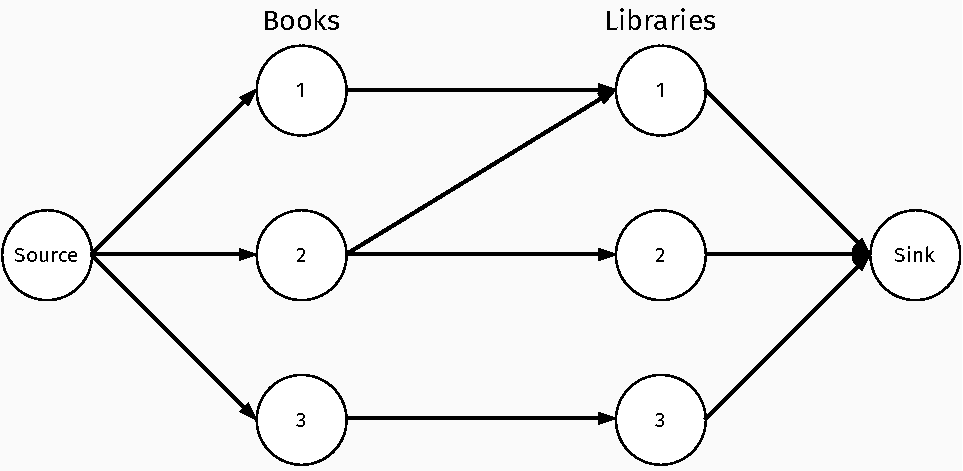
\includegraphics[width=0.8\textwidth,keepaspectratio]{../assets/bs/bs-graph-slides.pdf}
    \caption{Assignment Problem Modeled as a Bipartite Graph}
  \end{figure}
\end{frame}

\begin{frame}{Modeling --- Two-Phase Approach Local Moves}
  After the book assignment the solution can be further improved through
  the following~\alert{local moves}:
  \begin{enumerate}
    \item \textbf{Reverse the sign-up order} between two libraries.
    \item \textbf{Change the positions of two libraries} in the order adjusting the
          sign-up times of every library in between.
    \item \textbf{Select one library to remove and add another library} that is not
          currently considered in that position, if possible.
  \end{enumerate}
\end{frame}

\begin{frame}{Results}
  The best objective values for the five instance of this problem were obtained using the
  \textbf{two-phase} approach, as illustrated in the table below:

  \begin{table}[ht]
    \centering
    \begin{tabular}{@{\extracolsep{4pt}}lcc@{\extracolsep{4pt}}}
      \toprule
      Instance                           & Objective Value & Best Known Objective Value \\ \midrule
      \textquote{Read On}                & \num{5822900}   & \num{5822900}              \\
      \textquote{Incunabula}             & \num{5689822}   & \num{5690888}              \\
      \textquote{Tough Choices}          & \num{5028530}   & \num{5107113}              \\
      \textquote{So many books}          & \num{5208455}   & \num{5237345}              \\
      \textquote{Libraries of the world} & \num{5328034}   & \num{5348248}              \\
      \bottomrule
    \end{tabular}
    \caption{Book Scanning Best Results}
  \end{table}

  Remarkably, this objective value would have placed us in~\textbf{33rd}
  place~(out of 10716 teams) on the competition leaderboard.
\end{frame}
  \caption{\acrlong{beam-search}}
  \label{algorithm:beam-search}
\end{algorithm}

The pseudocode assumes that the~\texttt{Branch} function generates the set of
all potential (partial) solutions achieved by incorporating components from the
ground set that are not currently part of the solution. It is worth noting that,
since the solution is constructed incrementally, the solutions obtained through
branching might not always be feasible.~As a result, an additional step for
feasibility verification is required before updating the best solution~($s$)
identified during the search process.~Likewise, a similar check is carried
out for the empty solution, as its feasibility can vary depending on the
specific problem being addressed.

It is important to emphasize that the~\emph{beam width} parameter directly
influences the quality of the solutions discovered.~Smaller values might lead to
premature convergence to a local optimum, while larger values, although capable
of producing better-quality solutions, could lead to increased memory and
computational requirements.~Futhermore, the effectiveness of
this~\acrshort{meta-heuristic} is also closely linked to the quality of the
upper bound function.

\subsection{Greedy Randomized Adaptive Search Procedure}
\label{subsec:grasp}

\acrfull{grasp}~\cite{resende2010greedya,outeiro2021application,blum2003metaheuristics}
is a stochastic,~\acrshort{constructive-search}
and~\acrshort{local-search},~\acrshort{meta-heuristic} that iteratively builds
solutions by sequencing a construction phase with an optional local search phase.~The
construction phase begins with an empty solution and iteratively adds a new
component at each step. This component is chosen at random from a
\emph{restricted candidate list} of components. This list consists of the best
available components for extending the current (partial) solution, based on
either a heuristic value or an upper bound.~Additionally, there's an option to
apply a local search phase to the partial solution obtained during the
construction phase. The goal of this local search is to further exploit the
solution, with algorithm concluding when some predefined stopping criteria are
met.~The provided pseudocode in~\Cref{algorithm:grasp} offers an overview of how the
\acrshort{grasp} algorithm works.

It is important to highlight that this meta-heuristic, provides a means of
controlling the balance between randomization and greediness in solution
construction (\texttt{GreedyRandomizedConstruction}). This control is
achieved through the parameter $\alpha$, which serves as a threshold for the
quality of solutions within the candidate list.~Specifically, when $\alpha = 1$,
the construction process is entirely random, and all possible components are
included in the candidate list, regardless of their quality.~Conversely, with
$\alpha = 0$, only the components with the optimal heuristic or bound value,
will be selected at random, rendering this~\acrshort{meta-heuristic} more
greedy. It is worth noting that the inclusion of the optional local search step
(\texttt{LocalSearch}) can significantly enhance the quality of the randomized
greedy process. However, the crux of fine-tuning lies in determining an
appropriate value for $\alpha$.

\begin{algorithm}
  % Greedy Randomized Adaptive Search Procedure (algorithm2e pseudocode)

\KwIn{Objective Function ($f$)}
\KwOut{Solution ($s^{*}$).}

\SetKwFunction{GreedyRandomizedConstruction}{\texttt{GreedyRandomizedConstruction}}
\SetKwFunction{LocalSearch}{\texttt{LocalSearch}}

$s^{*}$ $\gets$ $\emptyset$\;
\While{\texttt{stopping criteria not met}}{
  $s$ $\gets$ \GreedyRandomizedConstruction{}\;
  $s$ $\gets$ \LocalSearch{$s$}\;
  \If{$f(s)$ > $f(s^{*})$}{
    $s^{*}$ $\gets$ $s$\;
  }
}
\Return{$s^{*}$}
  \caption{\acrlong{grasp}}
  \label{algorithm:grasp}
\end{algorithm}

\subsection{Iterated Greedy}
\label{subsec:iterated-greedy}

\acrfull{iterated-greedy}~\cite{stutzle2018iterated,outeiro2021application} is a
\acrshort{constructive-search} trajectory~\acrshort{meta-heuristic} that
revolves around the concept of iteratively destroying a solution and
subsequently reconstructing it to break free from local optima. In its basic
form, this \acrshort{meta-heuristic} begins by constructing an initial solution,
for example through a randomized greedy approach. Subsequently, it proceeds to
remove one or more randomly chosen solution components before initiating the
construction process anew. This sequence of operations continues until some
predefined stopping criteria are satisfied.

Some less-common variations of this algorithm incorporate local search methods
to further exploit the solution following the construction phase. Furthermore,
certain versions of this~\acrshort{meta-heuristic}, as detailed in the
literature~\cite{stutzle2018iterated}, implement an acceptance criterion that
probabilistically permits the acceptance of solutions of inferior quality, akin
to the mechanisms employed in~\acrshort{simulated-annealing}, which will be
elaborated upon in~\Cref{subsec:simulated-annealing}.

As an illustration, the pseudocode for an ~\acrshort{iterated-greedy} algorithm
utilizing a randomized greedy strategy, is outlined
in~\Cref{algorithm:iterated-greedy}. Here, the functions \texttt{Construct}
and~\texttt{Destruct} signify the approach used for (re-)constructing and
destroying a solution, respectively.

\begin{algorithm}
  % Iterated Greedy (algorithm2e pseudocode)

\KwIn{Objective Function ($f$), Upper Bound Function($\Phi_{ub}$)}
\KwOut{Solution ($s^{*})$}

\SetKwFunction{Destruct}{\texttt{Destruct}}
\SetKwFunction{Construct}{\texttt{Construct}}
\SetKwFunction{LocalSearch}{\texttt{LocalSearch}}
\SetKwFunction{Accept}{\texttt{Accept}}

$s^{*}$ $\gets$ \Construct($\emptyset, \Phi_{ub}$)\;
\While{\texttt{stopping criteria not met}}{
  $s$ $\gets$ \Destruct{$s^{*}$}\;
  $s$ $\gets$ \Construct{$s, \Phi_{ub}$}\;
  \If{$s\ $ \texttt{is feasible} $\land$ $f(s) > f(s^{*})$}{
    $s^{*}$ $\gets$ $s'$\;
  }
}
  \caption{\acrlong{iterated-greedy}}
  \label{algorithm:iterated-greedy}
\end{algorithm}

\subsection{Ant Colony Optimization}
\label{subsec:aco}

\acrfull{aco}~\cite{dorigo2010anta,stutzle1999maxmin,luke2013essentialsa,blum2003metaheuristics}
is a stochastic population based,~\acrshort{constructive-search}
and~\acrshort{local-search},~\acrshort{meta-heuristic} that is inspired by the
foraging behavior of ants, which in the context algorithm represent (partial)
solutions undergoing construction.

The algorithm simulates the movement of~\textit{ants} through the search space,
where each ant constructs a solution by making a sequence of probabilistic
choices based on the~\textit{pheromone} trail left by previous ants and other
heuristic information. Notably, the pheromones, associated with the components
$c_{i}$ of the ground set $\mathcal{G}$, weigh the relevance of the integration
of a specific component in a solution during the construction process.
Moreover, the~\textit{pheromones} are associated with each component of the
ground set, and in practice consist in a parametrized probabilistic model.

One of the key features of~\acrshort{aco} is the incorporation of a learning component
through the use of a pheromone update rule that adapts the pheromone trail based
on the quality of the solutions constructed by the ants, with the aim of guiding
the ants towards better solutions over subsequent iterations. As such, the
algorithm requires the tuning of several parameters such as the pheromone
evaporation rate, the choice of the pheromone update rule, and the
initialization of the pheromone model. Notably, there are different models
which gave origin to many variations of this~\acrshort{meta-heuristic}.
The pseudocode provided in~\Cref{algorithm:aco} illustrates this~\acrshort{meta-heuristic}.

\begin{algorithm}
  % Ant Colony Optimization (algorithm2e pseudocode)

\KwIn{Pheromone Update Rule ($\mathcal{R}$), Pheromone Values ($\vec{\tau}$), Evaporation Rate ($\alpha$)}
\KwOut{Solution ($s$)}

\SetKwFunction{AntBasedSolutionConstruction}{\texttt{AntBasedSolutionConstruction}}
\SetKwFunction{PheromoneUpdate}{\texttt{PheromoneUpdate}}
\SetKwFunction{LocalSearch}{\texttt{LocalSearch}}

$s \gets$ $s'$\;
$bobj$ $\gets$ $-\infty$\;
$\mathcal{S} \gets \{ \emptyset \}$\;

\If{ $s\ $ \texttt{is feasible}}{
  $bobj$ $\gets$ $f(s)$\;
}

\While{\texttt{not stopping criteria met}}{
  $\mathcal{S}$ $\gets$ \AntBasedSolutionConstruction{$\mathcal{S}$, $\vec{\tau}$}\;
  $\mathcal{S}$ $\gets$ \LocalSearch{$\mathcal{S}$} \Comment*[f]{Optional} \;
  $s'$ $\gets$ $\underset{s'\ \in\ \mathcal{S}}{\argmax}\ f(s')$ \Comment*[f]{Select best solution}\;
  \If{$f(s')$ > $bobj$}{
    $s \gets s'$\;
    $bobj$ $\gets$ $f(s')$\;
  }
  $\mathcal{S} \gets$ \PheromoneUpdate{$\mathcal{S}$, $\mathcal{R}$, $\vec{\tau}$, $\alpha$}\;
}
\Return{$s^{*}$}
  \caption{\acrlong{aco}}
  \label{algorithm:aco}
\end{algorithm}

In summary, the~\acrshort{aco} meta-heuristic can be described as a process that
comprises of a solution construction
phase~(\texttt{AntBasedSolutionConstruction}), in which each solution
of the population is constructed using both the~\textit{pheromone model} and
heuristic information, followed by an optional phase of exploiting these
solutions through local search~(\texttt{LocalSearch}), and culminating
in a pheromone update phase~(\texttt{PheromoneUpdate}). This process is
then repeated for multiple iterations, until certain stopping criteria is met.

\subsection{Hill-Climbing}
\label{subsec:hill-climbing}

\acrfull{hill-climbing}~\cite{luke2013essentialsa,vieira2009uma} is a simple
stochastic,~\acrshort{local-search} trajectory~\acrshort{meta-heuristic} that
works by iteratively attempting to improve a starting solution through a
sequence of incremental changes,~\ie{}, by selecting the solution in the
neighborhood that yields the best increment with respect to the objective value.
This process terminates when the local optimal solution is found or another
stopping criteria is met. Despite the simplicity of this method it is worth
noting that, due to the inherent greedy choice of the best at each step this
approach is susceptible to getting trapped in local optima. For illustration
purposes the pseudocode of simple version of an~\acrshort{hill-climbing}
algorithm is shown in~\Cref{algorithm:hill-climbing}.

\begin{algorithm}
  % Hill Climbing (algorithm2e pseudocode)

\KwIn{Solution ($s$), Objective Function ($f$)}
\KwOut{Solution ($s$)}

\SetKwFunction{Perturb}{\texttt{Perturb}}

\While{ \texttt{stopping criteria not met} }{
  $s'$ $\gets$ \Perturb{$s$}\;
  \If{$f(s') > f(s)$}{
    $s$ $\gets$ $s'$\;
  }
}
\Return{ $s$ }
  \caption{\acrlong{hill-climbing}}
  \label{algorithm:hill-climbing}
\end{algorithm}

It is worth noting that the presented algorithm's effectiveness is rooted in the
efficiency of a random process, which strives to improve solution quality
through a sequence of random local move attempts (\texttt{ApplyRandomLocalMove} function).
Nevertheless, there exist two noteworthy variations that more thoroughly explore
the solution's neighborhood and take steps in the direction of the most
substantial improvement. These are commonly known as~\acrfull{first-improvement}
and~\acrfull{best-improvement}. The latter is also known in the literature as
\textit{steepest ascent}~\acrshort{hill-climbing}~\cite{luke2013essentialsa}.

In a~\acrshort{first-improvement} approach, the first random neighboring solution that
improves the current solution's quality is retained. Conversely, in a
\acrshort{best-improvement} scenario, the entire neighborhood of the current
solution is examined, and the best neighboring solution is selected for the
subsequent iteration.

\subsection{Iterated Local Search}
\label{subsec:iterated-local-search}

\acrfull{iterated-local-search}~\cite{lourenco2010iterateda,luke2013essentialsa,blum2003metaheuristics}
is a stochastic \acrshort{local-search} trajectory~\acrshort{meta-heuristic} that
extends the \acrshort{hill-climbing} method. This algorithm operates through a
series of iterations, where each iteration aims to explore a solution by
applying a~\acrshort{local-search} procedure,
typically~\acrshort{first-improvement}. When an improvement is achieved, the
best solution found is retained and serves as the reference solution for
subsequent iterations. This iterative process continues until the algorithm
either converges to the local optimum or meets predefined stopping criteria.

An integral feature of the~\acrshort{iterated-local-search} is the introduction
of a perturbation step at the end of each iteration. This perturbation injects
controlled randomness into the current solution, allowing for exploration of
different regions within the search space. This exploration aids in preventing
the algorithm from becoming stuck in local optima.~Notably, other many
variations of this algorithm exist, with certain versions incorporating an
archive mechanism to store starting solutions for each iteration. This approach
helps prevent repeated exploration of the same regions within the search space.

The core framework of the \acrshort{iterated-local-search} algorithm is
illustrated in Algorithm~\ref{algorithm:iterated-local-search}. The parameter
$k$ in the \texttt{Perturb} function represents the \textit{kick strength},
determining the intensity of the perturbation movement, and can be
adjusted accordingly.

\begin{algorithm}
  % Constructive Search Procedure (algorithm2e pseudocode)

\KwIn{Solution ($s$), Kick Strength ($k$), Objective Function ($f$)}
\KwOut{Solution ($s$).}

\SetKwFunction{Perturb}{\texttt{Perturb}}
\SetKwFunction{LocalSearch}{\texttt{LocalSearch}}

\While{\texttt{stopping criteria not met}}{
  $s'$ $\gets$ \LocalSearch{$s$}\;
  $s'$ $\gets$ \Perturb{$s', k$}\;
  \If{$f(s') > f(s$)}{
    $s$ $\gets$ $s'$\;
  }
}
\Return{$s$}
  \caption{\acrlong{iterated-local-search}}
  \label{algorithm:iterated-local-search}
\end{algorithm}

\subsection{Simulated Annealing}
\label{subsec:simulated-annealing}

\acrfull{simulated-annealing}~\cite{kirkpatrick1983optimization,nikolaev2010simulateda,eglese1990simulated}
is a stochastic,~\acrshort{local-search} trajectory~\acrshort{meta-heuristic}
that draws inspiration from the \emph{annealing} process in metallurgy. The core
concept adopted from metallurgy and applied to the algorithmic context is the
notion of accepting poorer quality solutions in the early stages of the search
and gradually tightening the acceptance criteria as the search progresses. This
strategy is based on the understanding that in the initial phases, accepting
suboptimal solutions as the best available option promotes exploration of the
search space. As the search advances towards its final stages, the emphasis
shifts towards convergence to a local optimum, favoring exploitation.

Essentially,~\acrshort{simulated-annealing} works by iteratively applying small
perturbations to a candidate solution in order to enhance it. The algorithm
accepts or rejects these new solutions based on their quality and a probability
function that emulates the cooling process of a metal.~This probability function
depends on a temperature parameter, which decreases as the algorithm proceeds,
causing the acceptance probability of worst solutions to decrease as well.
Ultimately, the algorithm halts when further improvements to the solution are no
longer feasible or when predefined stopping criteria are met.

The details of the~\acrshort{simulated-annealing} algorithm are illustrated in the
pseudocode provided in~\Cref{algorithm:simulated-annealing}.

\begin{algorithm}
  % Simulated Annealing (algorithm2e pseudocode)

\KwIn{Solution ($s$), Initial Temperature ($t_{0}$), Cooling Rate ($\alpha$), Objective Function ($f$) }
\KwOut{Solution ($s$)}

\SetKwFunction{Random}{\texttt{Random}}
\SetKwFunction{Perturb}{\texttt{Perturb}}

$t \gets t_{0}$\;
\While{\texttt{stopping criteria not met}}{
  $s' \gets$ \Perturb{$s$}\;
  $\delta$ $\gets$ $f(s)$ - $f(s')$\;
  \If{$\delta < 0$ $\lor$ \Random{$0, 1$} $ < $ $e^{-\frac{\delta}{t}}$}{
    $s$ $\gets$ $s'$\;
  }
  $t$ $\gets$ $t \cdot \alpha$\;
}
\Return{$s$}
  \caption{\acrlong{simulated-annealing}}
  \label{algorithm:simulated-annealing}
\end{algorithm}

Importantly, the~\acrshort{simulated-annealing} algorithm is tunable, allowing
for parameter adjustments to suit the specific problem at hand.~Parameters such
as the initial temperature, cooling function, and acceptance criteria can be
fine-tuned for optimal performance.~In~\Cref{algorithm:simulated-annealing}, the
acceptance criteria is defined using an exponential function, while the cooling
process is held constant and governed by the parameter $\alpha$.

\subsection{Tabu Search}
\label{subsec:tabu-search}

\acrfull{tabu-search}~\cite{glover1999tabu,gendreau2010tabua,luke2013essentialsa}
is a stochastic,~\acrshort{local-search}~trajectory~\acrshort{meta-heuristic}
that incorporates the use of a memory to aid the search process.

In essence,the \acrshort{tabu-search} algorithm operates by conducting an
iterative exploration of the solution space through the repeated application of
a series of \acrshort{best-improvement} procedures. During each step, the best
solution is updated and added to a list of recently visited solutions known as
the \emph{tabu list}.~The tabu list has a predefined size and serves as a
short-term memory mechanism.~This approach aims to prevent the algorithm from
revisiting solutions that have been explored before, thereby avoiding premature
convergence to local optima.~By incetivizing exploration of new regions in the
search space, the algorithm enhances its ability to find better
solutions.~Similar to other \acrshort{local-search} meta-heuristics, the
\acrfull{tabu-search} algorithm terminates when no further improvement to the
solution is achievable.

The pseudocode in~\Cref{algorithm:tabu-search} illustrates a simple version of
this meta-heuristic.

\begin{algorithm}
  % Tabu Search (algorithm2e pseudocode)

\KwIn{Solution ($s'$), Tabu Length ($l_{max}$), Objective Function ($f$)}
\KwOut{Solution ($s^{*}$)}

\SetKwFunction{Oldest}{\texttt{Oldest}}

$s^{*} \gets$ $s'$\;
$\mathcal{T}$ $\gets$ $\{ \emptyset \}$\;
\While{\texttt{stopping criteria not met}}{
  $s$ $\gets$ $\underset{s\ \in\ \mathcal{N}(s) \backslash \mathcal{T}}{\argmax}\ f(s)$ \Comment*[f]{Select best neighbor $s \notin \mathcal{T}$}\;
  \If{$f(s) > f(s^{*})$}{
    $s^{*}$ $\gets$ $s$\;
    $\mathcal{T} \gets \mathcal{T} \cup \{s\}$\;
  }
  \If{$\left\lvert \mathcal{T} \right\rvert$ $>$ $l_{\max}$} {
    $\mathcal{T}$ $\gets$ $\mathcal{T}\ \setminus $ \Oldest{$\mathcal{T}$}\;
  }
}
\Return{$s^{*}$}
  \caption{\acrlong{tabu-search}}
  \label{algorithm:tabu-search}
\end{algorithm}

Notably, the size and duration of the tabu list ($l_{\max}$), as well as the
rules for adding and removing solutions from the list, are user-specified
parameters that need to be fine-tuned for each problem.~Additionally, a common
criterion for the removal of an element from the tabu list is based on its age.
This aspect related to age-based removal is depicted
in~\Cref{algorithm:tabu-search} through the utilization of the~\texttt{Oldest}
function, which retrieves the oldest solution stored within the tabu list.

\subsection{Outline}
\label{subsec:Outline}

In this section, we provided a concise overview of well-known state-of-the-art
meta-heuristic algorithms that hold relevance to our study. Our intention was to
offer the reader a general understanding of the conceptual foundation behind each
algorithm, without delving into an exhaustive exploration. Furthermore, we
categorized each meta-heuristic based on the employed search strategy
(\acrshort{constructive-search} or~\acrshort{local-search}), the utilization of a memory archive for
solutions, and the state size (\textit{Population} vs. \textit{Trajectory}).

The~\Cref{tab:meta-heuristics-summary} presents a succinct summary of various
meta-heuristic methods, organized according to these properties.

\begin{table}[ht]
  In the literature, a multitude of meta-heuristic algorithms have emerged over
the years, exploring various ideas to guide the search
process~\cite{osman1996metaheuristics}. These encompass strategies that narrow
the search space to promising regions, enhance solutions in a greedy manner, or
utilize randomized and probabilistic techniques, some of which draw inspiration
from natural phenomena like collective behavior, natural selection, and physical
processes of materials.

However, the majority of state-of-the-art meta-heuristic algorithms can be
described by a few distinctive traits~\cite{blum2003metaheuristics} such as:

\begin{description}
  \item[\textbf{Search Strategy.}] This refers to the method used to find a
    solution.~It can be one of three main types: constructive, local, or a
    \emph{composite} approach that combines both strategies.

  \item[\textbf{Memoization.}] This concept involves maintaining a record or
    archive of previously explored solutions.~This record helps in identifying
    solutions that may be revisited or disregarded in subsequent stages of the
    optimization process.

  \item[\textbf{State Size.}] This pertains to the number of solutions being
    evolved during the construction phase.~In~\emph{population methods}, multiple
    solutions are worked with at each iteration, while in~\emph{trajectory methods} (single-state),
    only a single solution is improved at a time.
\end{description}

In this section, we will offer a brief overview of select state-of-the-art
\acrshort{meta-heuristic} algorithms, which encapsulate all the above properties
and will be utilized and implemented in the context of this work.

\subsection{Beam Search}
\label{subsec:beam-search}

\acrfull{beam-search}~\cite{ow1988filtered,outeiro2021application} is a
\acrshort{constructive-search} population~\acrfull{meta-heuristic} inspired by
the~\emph{breadth-first search} algorithm~\cite{papadimitriou1998combinatorial}.
However, it deviates from the conventional practice of expanding all solutions
in the search tree during each iteration. Instead, this technique maintains a
fixed-size archive of previous solutions, which are expanded at each
step~(\textit{beam}). Subsequently, the expanded solutions undergo filtering,
and only the best solutions, determined based on heuristic information or bound
values, are retained within the archive. These selected solutions act as the
starting points for the next iteration. It is important to acknowledge that the
size of this archive, and consequently the number of solutions filtered at each
step, is dictated by a parameter referred to as the~\emph{beam width}.

The construction process of~\acrshort{beam-search} terminates either when there
are no more candidate solutions to expand or when other predetermined stopping
criteria are satisfied. For illustration purposes, the pseudocode for
\acrshort{beam-search} is presented in \Cref{algorithm:beam-search}.
In this context, the notation $\argmax_{w}$ is employed to introduce the concept
of selecting the top $w$ elements from a given set.

\begin{algorithm}[h]
  \begin{frame}{Problem}
  This problem entails the setup of scanning pipeline for books.

  \begin{itemize}
    \item There are libraries housing various books. Before any scanning can commence, each
          library needs to register for the scanning process. Once registered, each
          library is allowed to scan a certain number of books daily, until global deadline.
    \item Only one library can undergo the sign-up process at any given time.
    \item Each book, when scanned, contributes a specific score.
  \end{itemize}

\end{frame}

\begin{frame}{Example --- Book Scanning}
  \begin{figure}[h]
    \centering
    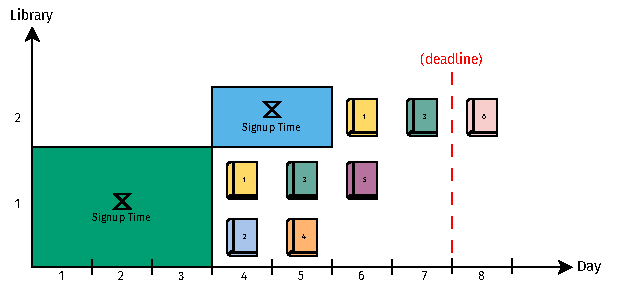
\includegraphics[width=0.8\textwidth,keepaspectratio]{../assets/bs/bs-example-slides.pdf}
    \caption{Book Scanning Example}
  \end{figure}

  \begin{table}[ht]
    \centering
    \begin{tabular}{ccccccc}
      \toprule
      \textbf{Book}  & 1 & 2 & 3 & 4 & 5 & 6 \\ \midrule
      \textbf{Score} & 3 & 1 & 5 & 4 & 7 & 1 \\
      \bottomrule
    \end{tabular}
    \caption{Book Scores}
  \end{table}
\end{frame}

\begin{frame}{Problem Formulation}
  \begin{equation*}
    \begin{aligned}
      \max\ f(x) =\  & \sum_{b = 1}^{\mathcal{B}}{s_{b} \cdot \min\left(\sum_{i = 1}^{\mathcal{I}}{x_{b, \phi_{i}^\mathcal{I}}} , 1\right)}                                                                     \\
      \text{s.t }    & \sum_{b = 1}^{\mathcal{B}}{x_{b, \phi_{i}^\mathcal{I}}} \leq r_{i} \cdot \left(\mathcal{D} - \sum_{k = 1}^{i}{t_{\phi_{k}^\mathcal{I}}} \right) \quad \forall i = 1, \ldots, \mathcal{I} \\
                     & \sum_{i = 1}^{\mathcal{I}}{t_{\phi_{i}^\mathcal{I}}} \leq \mathcal{D}                                                                                                                    \\
    \end{aligned}
  \end{equation*}
  Where,
  \begin{itemize}
    \item $\mathcal{B}$ is the number of books.
    \item $\mathcal{D}$ is the global deadline.
    \item $\mathcal{I}$ and $\phi^\mathcal{I}$ are the number and order of signed-up libraries.
    \item $t_{i}$ and $r_{i}$ are the sign-up time and book scanning rate of library $i$.
    \item $s_{b}$ is the score of book $b$.
    \item $x_{b,i}$ is binary variable indicating if a book, $b$, is assigned (1) or not (0) to library $i$.
  \end{itemize}
\end{frame}


\begin{frame}{Example --- Objective}
  \begin{figure}[h]
    \centering
    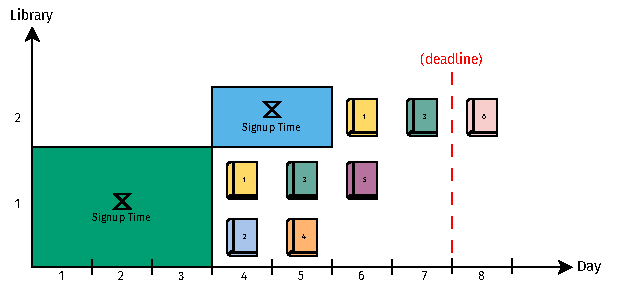
\includegraphics[width=0.8\textwidth,keepaspectratio]{../assets/bs/bs-example-slides.pdf}
  \end{figure}
  \begin{table}
    \begin{tabular}{cc}
      \begin{minipage}{0.5\textwidth}
        \begin{table}[ht]
          \centering
          \begin{tabular}{ccccccc}
            \toprule
            \textbf{Book}  & 1          & 2          & 3          & 4          & 5          & 6 \\ \midrule
            \textbf{Score} & \textbf{3} & \textbf{1} & \textbf{5} & \textbf{4} & \textbf{7} & 1 \\
            \bottomrule
          \end{tabular}
        \end{table}
      \end{minipage}
       &
      \begin{minipage}[b]{0.5\textwidth}
        \centering
        \begin{equation*}
          f(x) = 3 + 1 + 5 + 4 + 7 = 20
        \end{equation*}
      \end{minipage}
    \end{tabular}
    \caption{Book Scores \& Objective Value}
  \end{table}
\end{frame}

\begin{frame}{Modeling --- Problem, Solution and Component}
  The~\alert{problem} is characterized by the set of all libraries available, along with
  their sign-up times, book shipping rate, and list of books that can be shipped,
  the scores for all the books, and the deadline.

  A~\alert{solution} is characterized by a collection of assignments of books
  to libraries and the order in which libraries are scanned.

  A~\alert{component} is characterized by a tuple containing a book and a library or
  a tuple containing two libraries (denoting the sign-up order).
\end{frame}

\begin{frame}{Modeling --- Construction Rules}
  Two component enumeration strategies were considered:
  \begin{itemize}
    \item \textbf{Standard:} Enumerate all the books that can be scanned by all signed-up libraries
          as well as all libraries that can be signed-up until the deadline.
    \item \textbf{Sequential:} Enumerate only the books of the last signed-up library and all the libraries
          that can still be signed-up.
  \end{itemize}
\end{frame}

\begin{frame}{Modeling -- Upper Bound}
  The upper bounds were devised for this problem are as follows:
  \begin{enumerate}
    \item \textbf{Individual Library Knapsacks:} In this approach, we treat the
          number of books each library can scan before the deadline as an individual
          knapsack. The bound value for each library is calculated as the sum of
          scores from the best books that are yet to be scanned. The
          global upper bound is then determined by summing up the bound values for
          each library.

    \item \textbf{Combined Knapsack for All Libraries:} Consider a single
          knapsack representing the total number of books that can be scanned by
          all libraries combined until the deadline.
  \end{enumerate}
\end{frame}

\begin{frame}{Modeling -- Local Moves}
  The~\alert{local moves} considered for this problem are:

  \begin{enumerate}
    \item \textbf{Adding a book} to the set of books to be scanned by a given library.
    \item \textbf{Removing a book} from the set of books that were going to be scanned by a library.
    \item \textbf{Swapping books between libraries}.
    \item \textbf{Removing a book} from the list of books to be scanned by a library and
          \textbf{adding that book to another library}. If possible, ~\textbf{replace the removed book} in
          the first library~\textbf{with another one} that is available there.
  \end{enumerate}
\end{frame}

\begin{frame}{Modeling --- Two-Phase Approach}
  Use a meta-heuristic to choose an order for the libraries and solve the book assignment problem optimally.

  Notably, the assignment problem can be modeled as bipartite graph and solved with any
  \textbf{min cost max-flow} solver.

  \begin{figure}[h]
    \centering
    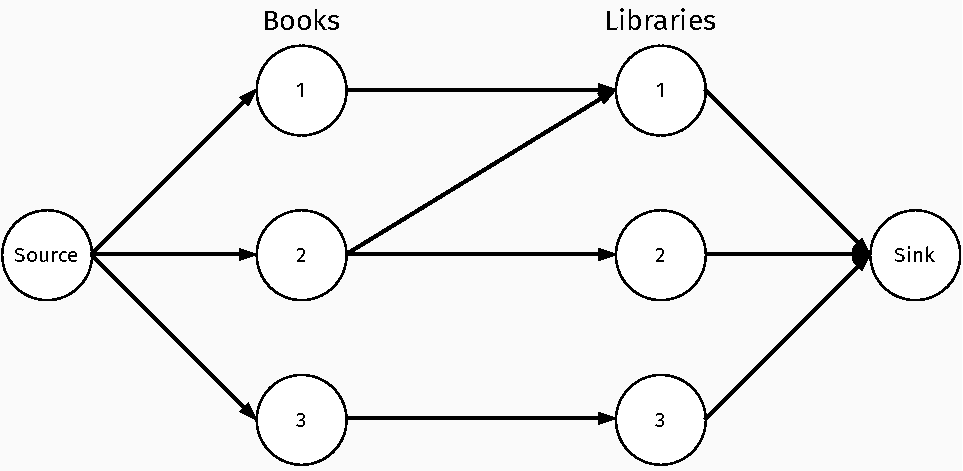
\includegraphics[width=0.8\textwidth,keepaspectratio]{../assets/bs/bs-graph-slides.pdf}
    \caption{Assignment Problem Modeled as a Bipartite Graph}
  \end{figure}
\end{frame}

\begin{frame}{Modeling --- Two-Phase Approach Local Moves}
  After the book assignment the solution can be further improved through
  the following~\alert{local moves}:
  \begin{enumerate}
    \item \textbf{Reverse the sign-up order} between two libraries.
    \item \textbf{Change the positions of two libraries} in the order adjusting the
          sign-up times of every library in between.
    \item \textbf{Select one library to remove and add another library} that is not
          currently considered in that position, if possible.
  \end{enumerate}
\end{frame}

\begin{frame}{Results}
  The best objective values for the five instance of this problem were obtained using the
  \textbf{two-phase} approach, as illustrated in the table below:

  \begin{table}[ht]
    \centering
    \begin{tabular}{@{\extracolsep{4pt}}lcc@{\extracolsep{4pt}}}
      \toprule
      Instance                           & Objective Value & Best Known Objective Value \\ \midrule
      \textquote{Read On}                & \num{5822900}   & \num{5822900}              \\
      \textquote{Incunabula}             & \num{5689822}   & \num{5690888}              \\
      \textquote{Tough Choices}          & \num{5028530}   & \num{5107113}              \\
      \textquote{So many books}          & \num{5208455}   & \num{5237345}              \\
      \textquote{Libraries of the world} & \num{5328034}   & \num{5348248}              \\
      \bottomrule
    \end{tabular}
    \caption{Book Scanning Best Results}
  \end{table}

  Remarkably, this objective value would have placed us in~\textbf{33rd}
  place~(out of 10716 teams) on the competition leaderboard.
\end{frame}
  \caption{\acrlong{beam-search}}
  \label{algorithm:beam-search}
\end{algorithm}

The pseudocode assumes that the~\texttt{Branch} function generates the set of
all potential (partial) solutions achieved by incorporating components from the
ground set that are not currently part of the solution. It is worth noting that,
since the solution is constructed incrementally, the solutions obtained through
branching might not always be feasible.~As a result, an additional step for
feasibility verification is required before updating the best solution~($s$)
identified during the search process.~Likewise, a similar check is carried
out for the empty solution, as its feasibility can vary depending on the
specific problem being addressed.

It is important to emphasize that the~\emph{beam width} parameter directly
influences the quality of the solutions discovered.~Smaller values might lead to
premature convergence to a local optimum, while larger values, although capable
of producing better-quality solutions, could lead to increased memory and
computational requirements.~Futhermore, the effectiveness of
this~\acrshort{meta-heuristic} is also closely linked to the quality of the
upper bound function.

\subsection{Greedy Randomized Adaptive Search Procedure}
\label{subsec:grasp}

\acrfull{grasp}~\cite{resende2010greedya,outeiro2021application,blum2003metaheuristics}
is a stochastic,~\acrshort{constructive-search}
and~\acrshort{local-search},~\acrshort{meta-heuristic} that iteratively builds
solutions by sequencing a construction phase with an optional local search phase.~The
construction phase begins with an empty solution and iteratively adds a new
component at each step. This component is chosen at random from a
\emph{restricted candidate list} of components. This list consists of the best
available components for extending the current (partial) solution, based on
either a heuristic value or an upper bound.~Additionally, there's an option to
apply a local search phase to the partial solution obtained during the
construction phase. The goal of this local search is to further exploit the
solution, with algorithm concluding when some predefined stopping criteria are
met.~The provided pseudocode in~\Cref{algorithm:grasp} offers an overview of how the
\acrshort{grasp} algorithm works.

It is important to highlight that this meta-heuristic, provides a means of
controlling the balance between randomization and greediness in solution
construction (\texttt{GreedyRandomizedConstruction}). This control is
achieved through the parameter $\alpha$, which serves as a threshold for the
quality of solutions within the candidate list.~Specifically, when $\alpha = 1$,
the construction process is entirely random, and all possible components are
included in the candidate list, regardless of their quality.~Conversely, with
$\alpha = 0$, only the components with the optimal heuristic or bound value,
will be selected at random, rendering this~\acrshort{meta-heuristic} more
greedy. It is worth noting that the inclusion of the optional local search step
(\texttt{LocalSearch}) can significantly enhance the quality of the randomized
greedy process. However, the crux of fine-tuning lies in determining an
appropriate value for $\alpha$.

\begin{algorithm}
  % Greedy Randomized Adaptive Search Procedure (algorithm2e pseudocode)

\KwIn{Objective Function ($f$)}
\KwOut{Solution ($s^{*}$).}

\SetKwFunction{GreedyRandomizedConstruction}{\texttt{GreedyRandomizedConstruction}}
\SetKwFunction{LocalSearch}{\texttt{LocalSearch}}

$s^{*}$ $\gets$ $\emptyset$\;
\While{\texttt{stopping criteria not met}}{
  $s$ $\gets$ \GreedyRandomizedConstruction{}\;
  $s$ $\gets$ \LocalSearch{$s$}\;
  \If{$f(s)$ > $f(s^{*})$}{
    $s^{*}$ $\gets$ $s$\;
  }
}
\Return{$s^{*}$}
  \caption{\acrlong{grasp}}
  \label{algorithm:grasp}
\end{algorithm}

\subsection{Iterated Greedy}
\label{subsec:iterated-greedy}

\acrfull{iterated-greedy}~\cite{stutzle2018iterated,outeiro2021application} is a
\acrshort{constructive-search} trajectory~\acrshort{meta-heuristic} that
revolves around the concept of iteratively destroying a solution and
subsequently reconstructing it to break free from local optima. In its basic
form, this \acrshort{meta-heuristic} begins by constructing an initial solution,
for example through a randomized greedy approach. Subsequently, it proceeds to
remove one or more randomly chosen solution components before initiating the
construction process anew. This sequence of operations continues until some
predefined stopping criteria are satisfied.

Some less-common variations of this algorithm incorporate local search methods
to further exploit the solution following the construction phase. Furthermore,
certain versions of this~\acrshort{meta-heuristic}, as detailed in the
literature~\cite{stutzle2018iterated}, implement an acceptance criterion that
probabilistically permits the acceptance of solutions of inferior quality, akin
to the mechanisms employed in~\acrshort{simulated-annealing}, which will be
elaborated upon in~\Cref{subsec:simulated-annealing}.

As an illustration, the pseudocode for an ~\acrshort{iterated-greedy} algorithm
utilizing a randomized greedy strategy, is outlined
in~\Cref{algorithm:iterated-greedy}. Here, the functions \texttt{Construct}
and~\texttt{Destruct} signify the approach used for (re-)constructing and
destroying a solution, respectively.

\begin{algorithm}
  % Iterated Greedy (algorithm2e pseudocode)

\KwIn{Objective Function ($f$), Upper Bound Function($\Phi_{ub}$)}
\KwOut{Solution ($s^{*})$}

\SetKwFunction{Destruct}{\texttt{Destruct}}
\SetKwFunction{Construct}{\texttt{Construct}}
\SetKwFunction{LocalSearch}{\texttt{LocalSearch}}
\SetKwFunction{Accept}{\texttt{Accept}}

$s^{*}$ $\gets$ \Construct($\emptyset, \Phi_{ub}$)\;
\While{\texttt{stopping criteria not met}}{
  $s$ $\gets$ \Destruct{$s^{*}$}\;
  $s$ $\gets$ \Construct{$s, \Phi_{ub}$}\;
  \If{$s\ $ \texttt{is feasible} $\land$ $f(s) > f(s^{*})$}{
    $s^{*}$ $\gets$ $s'$\;
  }
}
  \caption{\acrlong{iterated-greedy}}
  \label{algorithm:iterated-greedy}
\end{algorithm}

\subsection{Ant Colony Optimization}
\label{subsec:aco}

\acrfull{aco}~\cite{dorigo2010anta,stutzle1999maxmin,luke2013essentialsa,blum2003metaheuristics}
is a stochastic population based,~\acrshort{constructive-search}
and~\acrshort{local-search},~\acrshort{meta-heuristic} that is inspired by the
foraging behavior of ants, which in the context algorithm represent (partial)
solutions undergoing construction.

The algorithm simulates the movement of~\textit{ants} through the search space,
where each ant constructs a solution by making a sequence of probabilistic
choices based on the~\textit{pheromone} trail left by previous ants and other
heuristic information. Notably, the pheromones, associated with the components
$c_{i}$ of the ground set $\mathcal{G}$, weigh the relevance of the integration
of a specific component in a solution during the construction process.
Moreover, the~\textit{pheromones} are associated with each component of the
ground set, and in practice consist in a parametrized probabilistic model.

One of the key features of~\acrshort{aco} is the incorporation of a learning component
through the use of a pheromone update rule that adapts the pheromone trail based
on the quality of the solutions constructed by the ants, with the aim of guiding
the ants towards better solutions over subsequent iterations. As such, the
algorithm requires the tuning of several parameters such as the pheromone
evaporation rate, the choice of the pheromone update rule, and the
initialization of the pheromone model. Notably, there are different models
which gave origin to many variations of this~\acrshort{meta-heuristic}.
The pseudocode provided in~\Cref{algorithm:aco} illustrates this~\acrshort{meta-heuristic}.

\begin{algorithm}
  % Ant Colony Optimization (algorithm2e pseudocode)

\KwIn{Pheromone Update Rule ($\mathcal{R}$), Pheromone Values ($\vec{\tau}$), Evaporation Rate ($\alpha$)}
\KwOut{Solution ($s$)}

\SetKwFunction{AntBasedSolutionConstruction}{\texttt{AntBasedSolutionConstruction}}
\SetKwFunction{PheromoneUpdate}{\texttt{PheromoneUpdate}}
\SetKwFunction{LocalSearch}{\texttt{LocalSearch}}

$s \gets$ $s'$\;
$bobj$ $\gets$ $-\infty$\;
$\mathcal{S} \gets \{ \emptyset \}$\;

\If{ $s\ $ \texttt{is feasible}}{
  $bobj$ $\gets$ $f(s)$\;
}

\While{\texttt{not stopping criteria met}}{
  $\mathcal{S}$ $\gets$ \AntBasedSolutionConstruction{$\mathcal{S}$, $\vec{\tau}$}\;
  $\mathcal{S}$ $\gets$ \LocalSearch{$\mathcal{S}$} \Comment*[f]{Optional} \;
  $s'$ $\gets$ $\underset{s'\ \in\ \mathcal{S}}{\argmax}\ f(s')$ \Comment*[f]{Select best solution}\;
  \If{$f(s')$ > $bobj$}{
    $s \gets s'$\;
    $bobj$ $\gets$ $f(s')$\;
  }
  $\mathcal{S} \gets$ \PheromoneUpdate{$\mathcal{S}$, $\mathcal{R}$, $\vec{\tau}$, $\alpha$}\;
}
\Return{$s^{*}$}
  \caption{\acrlong{aco}}
  \label{algorithm:aco}
\end{algorithm}

In summary, the~\acrshort{aco} meta-heuristic can be described as a process that
comprises of a solution construction
phase~(\texttt{AntBasedSolutionConstruction}), in which each solution
of the population is constructed using both the~\textit{pheromone model} and
heuristic information, followed by an optional phase of exploiting these
solutions through local search~(\texttt{LocalSearch}), and culminating
in a pheromone update phase~(\texttt{PheromoneUpdate}). This process is
then repeated for multiple iterations, until certain stopping criteria is met.

\subsection{Hill-Climbing}
\label{subsec:hill-climbing}

\acrfull{hill-climbing}~\cite{luke2013essentialsa,vieira2009uma} is a simple
stochastic,~\acrshort{local-search} trajectory~\acrshort{meta-heuristic} that
works by iteratively attempting to improve a starting solution through a
sequence of incremental changes,~\ie{}, by selecting the solution in the
neighborhood that yields the best increment with respect to the objective value.
This process terminates when the local optimal solution is found or another
stopping criteria is met. Despite the simplicity of this method it is worth
noting that, due to the inherent greedy choice of the best at each step this
approach is susceptible to getting trapped in local optima. For illustration
purposes the pseudocode of simple version of an~\acrshort{hill-climbing}
algorithm is shown in~\Cref{algorithm:hill-climbing}.

\begin{algorithm}
  % Hill Climbing (algorithm2e pseudocode)

\KwIn{Solution ($s$), Objective Function ($f$)}
\KwOut{Solution ($s$)}

\SetKwFunction{Perturb}{\texttt{Perturb}}

\While{ \texttt{stopping criteria not met} }{
  $s'$ $\gets$ \Perturb{$s$}\;
  \If{$f(s') > f(s)$}{
    $s$ $\gets$ $s'$\;
  }
}
\Return{ $s$ }
  \caption{\acrlong{hill-climbing}}
  \label{algorithm:hill-climbing}
\end{algorithm}

It is worth noting that the presented algorithm's effectiveness is rooted in the
efficiency of a random process, which strives to improve solution quality
through a sequence of random local move attempts (\texttt{ApplyRandomLocalMove} function).
Nevertheless, there exist two noteworthy variations that more thoroughly explore
the solution's neighborhood and take steps in the direction of the most
substantial improvement. These are commonly known as~\acrfull{first-improvement}
and~\acrfull{best-improvement}. The latter is also known in the literature as
\textit{steepest ascent}~\acrshort{hill-climbing}~\cite{luke2013essentialsa}.

In a~\acrshort{first-improvement} approach, the first random neighboring solution that
improves the current solution's quality is retained. Conversely, in a
\acrshort{best-improvement} scenario, the entire neighborhood of the current
solution is examined, and the best neighboring solution is selected for the
subsequent iteration.

\subsection{Iterated Local Search}
\label{subsec:iterated-local-search}

\acrfull{iterated-local-search}~\cite{lourenco2010iterateda,luke2013essentialsa,blum2003metaheuristics}
is a stochastic \acrshort{local-search} trajectory~\acrshort{meta-heuristic} that
extends the \acrshort{hill-climbing} method. This algorithm operates through a
series of iterations, where each iteration aims to explore a solution by
applying a~\acrshort{local-search} procedure,
typically~\acrshort{first-improvement}. When an improvement is achieved, the
best solution found is retained and serves as the reference solution for
subsequent iterations. This iterative process continues until the algorithm
either converges to the local optimum or meets predefined stopping criteria.

An integral feature of the~\acrshort{iterated-local-search} is the introduction
of a perturbation step at the end of each iteration. This perturbation injects
controlled randomness into the current solution, allowing for exploration of
different regions within the search space. This exploration aids in preventing
the algorithm from becoming stuck in local optima.~Notably, other many
variations of this algorithm exist, with certain versions incorporating an
archive mechanism to store starting solutions for each iteration. This approach
helps prevent repeated exploration of the same regions within the search space.

The core framework of the \acrshort{iterated-local-search} algorithm is
illustrated in Algorithm~\ref{algorithm:iterated-local-search}. The parameter
$k$ in the \texttt{Perturb} function represents the \textit{kick strength},
determining the intensity of the perturbation movement, and can be
adjusted accordingly.

\begin{algorithm}
  % Constructive Search Procedure (algorithm2e pseudocode)

\KwIn{Solution ($s$), Kick Strength ($k$), Objective Function ($f$)}
\KwOut{Solution ($s$).}

\SetKwFunction{Perturb}{\texttt{Perturb}}
\SetKwFunction{LocalSearch}{\texttt{LocalSearch}}

\While{\texttt{stopping criteria not met}}{
  $s'$ $\gets$ \LocalSearch{$s$}\;
  $s'$ $\gets$ \Perturb{$s', k$}\;
  \If{$f(s') > f(s$)}{
    $s$ $\gets$ $s'$\;
  }
}
\Return{$s$}
  \caption{\acrlong{iterated-local-search}}
  \label{algorithm:iterated-local-search}
\end{algorithm}

\subsection{Simulated Annealing}
\label{subsec:simulated-annealing}

\acrfull{simulated-annealing}~\cite{kirkpatrick1983optimization,nikolaev2010simulateda,eglese1990simulated}
is a stochastic,~\acrshort{local-search} trajectory~\acrshort{meta-heuristic}
that draws inspiration from the \emph{annealing} process in metallurgy. The core
concept adopted from metallurgy and applied to the algorithmic context is the
notion of accepting poorer quality solutions in the early stages of the search
and gradually tightening the acceptance criteria as the search progresses. This
strategy is based on the understanding that in the initial phases, accepting
suboptimal solutions as the best available option promotes exploration of the
search space. As the search advances towards its final stages, the emphasis
shifts towards convergence to a local optimum, favoring exploitation.

Essentially,~\acrshort{simulated-annealing} works by iteratively applying small
perturbations to a candidate solution in order to enhance it. The algorithm
accepts or rejects these new solutions based on their quality and a probability
function that emulates the cooling process of a metal.~This probability function
depends on a temperature parameter, which decreases as the algorithm proceeds,
causing the acceptance probability of worst solutions to decrease as well.
Ultimately, the algorithm halts when further improvements to the solution are no
longer feasible or when predefined stopping criteria are met.

The details of the~\acrshort{simulated-annealing} algorithm are illustrated in the
pseudocode provided in~\Cref{algorithm:simulated-annealing}.

\begin{algorithm}
  % Simulated Annealing (algorithm2e pseudocode)

\KwIn{Solution ($s$), Initial Temperature ($t_{0}$), Cooling Rate ($\alpha$), Objective Function ($f$) }
\KwOut{Solution ($s$)}

\SetKwFunction{Random}{\texttt{Random}}
\SetKwFunction{Perturb}{\texttt{Perturb}}

$t \gets t_{0}$\;
\While{\texttt{stopping criteria not met}}{
  $s' \gets$ \Perturb{$s$}\;
  $\delta$ $\gets$ $f(s)$ - $f(s')$\;
  \If{$\delta < 0$ $\lor$ \Random{$0, 1$} $ < $ $e^{-\frac{\delta}{t}}$}{
    $s$ $\gets$ $s'$\;
  }
  $t$ $\gets$ $t \cdot \alpha$\;
}
\Return{$s$}
  \caption{\acrlong{simulated-annealing}}
  \label{algorithm:simulated-annealing}
\end{algorithm}

Importantly, the~\acrshort{simulated-annealing} algorithm is tunable, allowing
for parameter adjustments to suit the specific problem at hand.~Parameters such
as the initial temperature, cooling function, and acceptance criteria can be
fine-tuned for optimal performance.~In~\Cref{algorithm:simulated-annealing}, the
acceptance criteria is defined using an exponential function, while the cooling
process is held constant and governed by the parameter $\alpha$.

\subsection{Tabu Search}
\label{subsec:tabu-search}

\acrfull{tabu-search}~\cite{glover1999tabu,gendreau2010tabua,luke2013essentialsa}
is a stochastic,~\acrshort{local-search}~trajectory~\acrshort{meta-heuristic}
that incorporates the use of a memory to aid the search process.

In essence,the \acrshort{tabu-search} algorithm operates by conducting an
iterative exploration of the solution space through the repeated application of
a series of \acrshort{best-improvement} procedures. During each step, the best
solution is updated and added to a list of recently visited solutions known as
the \emph{tabu list}.~The tabu list has a predefined size and serves as a
short-term memory mechanism.~This approach aims to prevent the algorithm from
revisiting solutions that have been explored before, thereby avoiding premature
convergence to local optima.~By incetivizing exploration of new regions in the
search space, the algorithm enhances its ability to find better
solutions.~Similar to other \acrshort{local-search} meta-heuristics, the
\acrfull{tabu-search} algorithm terminates when no further improvement to the
solution is achievable.

The pseudocode in~\Cref{algorithm:tabu-search} illustrates a simple version of
this meta-heuristic.

\begin{algorithm}
  % Tabu Search (algorithm2e pseudocode)

\KwIn{Solution ($s'$), Tabu Length ($l_{max}$), Objective Function ($f$)}
\KwOut{Solution ($s^{*}$)}

\SetKwFunction{Oldest}{\texttt{Oldest}}

$s^{*} \gets$ $s'$\;
$\mathcal{T}$ $\gets$ $\{ \emptyset \}$\;
\While{\texttt{stopping criteria not met}}{
  $s$ $\gets$ $\underset{s\ \in\ \mathcal{N}(s) \backslash \mathcal{T}}{\argmax}\ f(s)$ \Comment*[f]{Select best neighbor $s \notin \mathcal{T}$}\;
  \If{$f(s) > f(s^{*})$}{
    $s^{*}$ $\gets$ $s$\;
    $\mathcal{T} \gets \mathcal{T} \cup \{s\}$\;
  }
  \If{$\left\lvert \mathcal{T} \right\rvert$ $>$ $l_{\max}$} {
    $\mathcal{T}$ $\gets$ $\mathcal{T}\ \setminus $ \Oldest{$\mathcal{T}$}\;
  }
}
\Return{$s^{*}$}
  \caption{\acrlong{tabu-search}}
  \label{algorithm:tabu-search}
\end{algorithm}

Notably, the size and duration of the tabu list ($l_{\max}$), as well as the
rules for adding and removing solutions from the list, are user-specified
parameters that need to be fine-tuned for each problem.~Additionally, a common
criterion for the removal of an element from the tabu list is based on its age.
This aspect related to age-based removal is depicted
in~\Cref{algorithm:tabu-search} through the utilization of the~\texttt{Oldest}
function, which retrieves the oldest solution stored within the tabu list.

\subsection{Outline}
\label{subsec:Outline}

In this section, we provided a concise overview of well-known state-of-the-art
meta-heuristic algorithms that hold relevance to our study. Our intention was to
offer the reader a general understanding of the conceptual foundation behind each
algorithm, without delving into an exhaustive exploration. Furthermore, we
categorized each meta-heuristic based on the employed search strategy
(\acrshort{constructive-search} or~\acrshort{local-search}), the utilization of a memory archive for
solutions, and the state size (\textit{Population} vs. \textit{Trajectory}).

The~\Cref{tab:meta-heuristics-summary} presents a succinct summary of various
meta-heuristic methods, organized according to these properties.

\begin{table}[ht]
  In the literature, a multitude of meta-heuristic algorithms have emerged over
the years, exploring various ideas to guide the search
process~\cite{osman1996metaheuristics}. These encompass strategies that narrow
the search space to promising regions, enhance solutions in a greedy manner, or
utilize randomized and probabilistic techniques, some of which draw inspiration
from natural phenomena like collective behavior, natural selection, and physical
processes of materials.

However, the majority of state-of-the-art meta-heuristic algorithms can be
described by a few distinctive traits~\cite{blum2003metaheuristics} such as:

\begin{description}
  \item[\textbf{Search Strategy.}] This refers to the method used to find a
    solution.~It can be one of three main types: constructive, local, or a
    \emph{composite} approach that combines both strategies.

  \item[\textbf{Memoization.}] This concept involves maintaining a record or
    archive of previously explored solutions.~This record helps in identifying
    solutions that may be revisited or disregarded in subsequent stages of the
    optimization process.

  \item[\textbf{State Size.}] This pertains to the number of solutions being
    evolved during the construction phase.~In~\emph{population methods}, multiple
    solutions are worked with at each iteration, while in~\emph{trajectory methods} (single-state),
    only a single solution is improved at a time.
\end{description}

In this section, we will offer a brief overview of select state-of-the-art
\acrshort{meta-heuristic} algorithms, which encapsulate all the above properties
and will be utilized and implemented in the context of this work.

\subsection{Beam Search}
\label{subsec:beam-search}

\acrfull{beam-search}~\cite{ow1988filtered,outeiro2021application} is a
\acrshort{constructive-search} population~\acrfull{meta-heuristic} inspired by
the~\emph{breadth-first search} algorithm~\cite{papadimitriou1998combinatorial}.
However, it deviates from the conventional practice of expanding all solutions
in the search tree during each iteration. Instead, this technique maintains a
fixed-size archive of previous solutions, which are expanded at each
step~(\textit{beam}). Subsequently, the expanded solutions undergo filtering,
and only the best solutions, determined based on heuristic information or bound
values, are retained within the archive. These selected solutions act as the
starting points for the next iteration. It is important to acknowledge that the
size of this archive, and consequently the number of solutions filtered at each
step, is dictated by a parameter referred to as the~\emph{beam width}.

The construction process of~\acrshort{beam-search} terminates either when there
are no more candidate solutions to expand or when other predetermined stopping
criteria are satisfied. For illustration purposes, the pseudocode for
\acrshort{beam-search} is presented in \Cref{algorithm:beam-search}.
In this context, the notation $\argmax_{w}$ is employed to introduce the concept
of selecting the top $w$ elements from a given set.

\begin{algorithm}[h]
  \begin{frame}{Problem}
  This problem entails the setup of scanning pipeline for books.

  \begin{itemize}
    \item There are libraries housing various books. Before any scanning can commence, each
          library needs to register for the scanning process. Once registered, each
          library is allowed to scan a certain number of books daily, until global deadline.
    \item Only one library can undergo the sign-up process at any given time.
    \item Each book, when scanned, contributes a specific score.
  \end{itemize}

\end{frame}

\begin{frame}{Example --- Book Scanning}
  \begin{figure}[h]
    \centering
    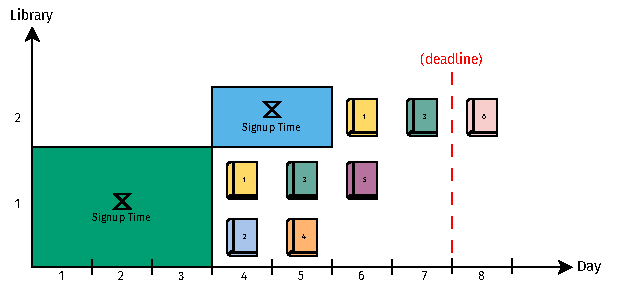
\includegraphics[width=0.8\textwidth,keepaspectratio]{../assets/bs/bs-example-slides.pdf}
    \caption{Book Scanning Example}
  \end{figure}

  \begin{table}[ht]
    \centering
    \begin{tabular}{ccccccc}
      \toprule
      \textbf{Book}  & 1 & 2 & 3 & 4 & 5 & 6 \\ \midrule
      \textbf{Score} & 3 & 1 & 5 & 4 & 7 & 1 \\
      \bottomrule
    \end{tabular}
    \caption{Book Scores}
  \end{table}
\end{frame}

\begin{frame}{Problem Formulation}
  \begin{equation*}
    \begin{aligned}
      \max\ f(x) =\  & \sum_{b = 1}^{\mathcal{B}}{s_{b} \cdot \min\left(\sum_{i = 1}^{\mathcal{I}}{x_{b, \phi_{i}^\mathcal{I}}} , 1\right)}                                                                     \\
      \text{s.t }    & \sum_{b = 1}^{\mathcal{B}}{x_{b, \phi_{i}^\mathcal{I}}} \leq r_{i} \cdot \left(\mathcal{D} - \sum_{k = 1}^{i}{t_{\phi_{k}^\mathcal{I}}} \right) \quad \forall i = 1, \ldots, \mathcal{I} \\
                     & \sum_{i = 1}^{\mathcal{I}}{t_{\phi_{i}^\mathcal{I}}} \leq \mathcal{D}                                                                                                                    \\
    \end{aligned}
  \end{equation*}
  Where,
  \begin{itemize}
    \item $\mathcal{B}$ is the number of books.
    \item $\mathcal{D}$ is the global deadline.
    \item $\mathcal{I}$ and $\phi^\mathcal{I}$ are the number and order of signed-up libraries.
    \item $t_{i}$ and $r_{i}$ are the sign-up time and book scanning rate of library $i$.
    \item $s_{b}$ is the score of book $b$.
    \item $x_{b,i}$ is binary variable indicating if a book, $b$, is assigned (1) or not (0) to library $i$.
  \end{itemize}
\end{frame}


\begin{frame}{Example --- Objective}
  \begin{figure}[h]
    \centering
    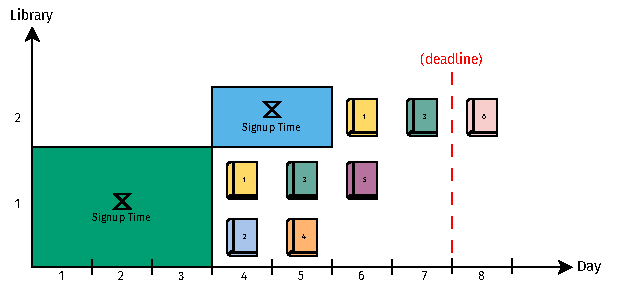
\includegraphics[width=0.8\textwidth,keepaspectratio]{../assets/bs/bs-example-slides.pdf}
  \end{figure}
  \begin{table}
    \begin{tabular}{cc}
      \begin{minipage}{0.5\textwidth}
        \begin{table}[ht]
          \centering
          \begin{tabular}{ccccccc}
            \toprule
            \textbf{Book}  & 1          & 2          & 3          & 4          & 5          & 6 \\ \midrule
            \textbf{Score} & \textbf{3} & \textbf{1} & \textbf{5} & \textbf{4} & \textbf{7} & 1 \\
            \bottomrule
          \end{tabular}
        \end{table}
      \end{minipage}
       &
      \begin{minipage}[b]{0.5\textwidth}
        \centering
        \begin{equation*}
          f(x) = 3 + 1 + 5 + 4 + 7 = 20
        \end{equation*}
      \end{minipage}
    \end{tabular}
    \caption{Book Scores \& Objective Value}
  \end{table}
\end{frame}

\begin{frame}{Modeling --- Problem, Solution and Component}
  The~\alert{problem} is characterized by the set of all libraries available, along with
  their sign-up times, book shipping rate, and list of books that can be shipped,
  the scores for all the books, and the deadline.

  A~\alert{solution} is characterized by a collection of assignments of books
  to libraries and the order in which libraries are scanned.

  A~\alert{component} is characterized by a tuple containing a book and a library or
  a tuple containing two libraries (denoting the sign-up order).
\end{frame}

\begin{frame}{Modeling --- Construction Rules}
  Two component enumeration strategies were considered:
  \begin{itemize}
    \item \textbf{Standard:} Enumerate all the books that can be scanned by all signed-up libraries
          as well as all libraries that can be signed-up until the deadline.
    \item \textbf{Sequential:} Enumerate only the books of the last signed-up library and all the libraries
          that can still be signed-up.
  \end{itemize}
\end{frame}

\begin{frame}{Modeling -- Upper Bound}
  The upper bounds were devised for this problem are as follows:
  \begin{enumerate}
    \item \textbf{Individual Library Knapsacks:} In this approach, we treat the
          number of books each library can scan before the deadline as an individual
          knapsack. The bound value for each library is calculated as the sum of
          scores from the best books that are yet to be scanned. The
          global upper bound is then determined by summing up the bound values for
          each library.

    \item \textbf{Combined Knapsack for All Libraries:} Consider a single
          knapsack representing the total number of books that can be scanned by
          all libraries combined until the deadline.
  \end{enumerate}
\end{frame}

\begin{frame}{Modeling -- Local Moves}
  The~\alert{local moves} considered for this problem are:

  \begin{enumerate}
    \item \textbf{Adding a book} to the set of books to be scanned by a given library.
    \item \textbf{Removing a book} from the set of books that were going to be scanned by a library.
    \item \textbf{Swapping books between libraries}.
    \item \textbf{Removing a book} from the list of books to be scanned by a library and
          \textbf{adding that book to another library}. If possible, ~\textbf{replace the removed book} in
          the first library~\textbf{with another one} that is available there.
  \end{enumerate}
\end{frame}

\begin{frame}{Modeling --- Two-Phase Approach}
  Use a meta-heuristic to choose an order for the libraries and solve the book assignment problem optimally.

  Notably, the assignment problem can be modeled as bipartite graph and solved with any
  \textbf{min cost max-flow} solver.

  \begin{figure}[h]
    \centering
    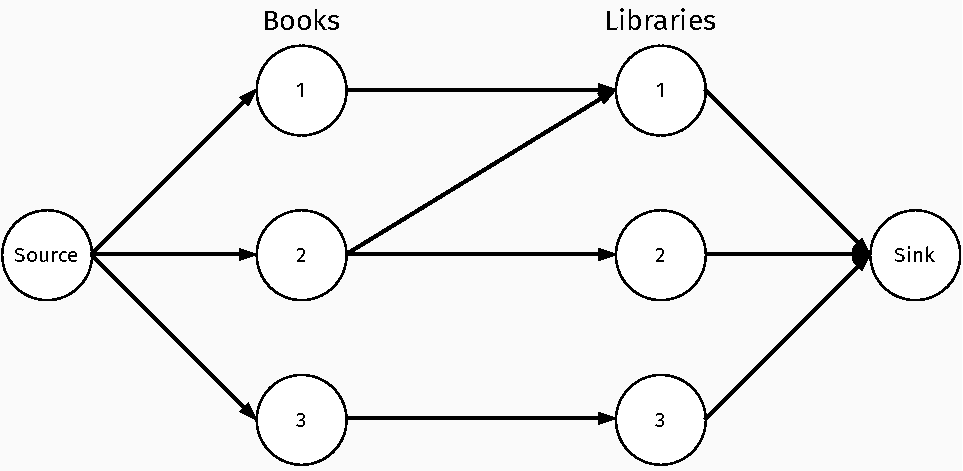
\includegraphics[width=0.8\textwidth,keepaspectratio]{../assets/bs/bs-graph-slides.pdf}
    \caption{Assignment Problem Modeled as a Bipartite Graph}
  \end{figure}
\end{frame}

\begin{frame}{Modeling --- Two-Phase Approach Local Moves}
  After the book assignment the solution can be further improved through
  the following~\alert{local moves}:
  \begin{enumerate}
    \item \textbf{Reverse the sign-up order} between two libraries.
    \item \textbf{Change the positions of two libraries} in the order adjusting the
          sign-up times of every library in between.
    \item \textbf{Select one library to remove and add another library} that is not
          currently considered in that position, if possible.
  \end{enumerate}
\end{frame}

\begin{frame}{Results}
  The best objective values for the five instance of this problem were obtained using the
  \textbf{two-phase} approach, as illustrated in the table below:

  \begin{table}[ht]
    \centering
    \begin{tabular}{@{\extracolsep{4pt}}lcc@{\extracolsep{4pt}}}
      \toprule
      Instance                           & Objective Value & Best Known Objective Value \\ \midrule
      \textquote{Read On}                & \num{5822900}   & \num{5822900}              \\
      \textquote{Incunabula}             & \num{5689822}   & \num{5690888}              \\
      \textquote{Tough Choices}          & \num{5028530}   & \num{5107113}              \\
      \textquote{So many books}          & \num{5208455}   & \num{5237345}              \\
      \textquote{Libraries of the world} & \num{5328034}   & \num{5348248}              \\
      \bottomrule
    \end{tabular}
    \caption{Book Scanning Best Results}
  \end{table}

  Remarkably, this objective value would have placed us in~\textbf{33rd}
  place~(out of 10716 teams) on the competition leaderboard.
\end{frame}
  \caption{\acrlong{beam-search}}
  \label{algorithm:beam-search}
\end{algorithm}

The pseudocode assumes that the~\texttt{Branch} function generates the set of
all potential (partial) solutions achieved by incorporating components from the
ground set that are not currently part of the solution. It is worth noting that,
since the solution is constructed incrementally, the solutions obtained through
branching might not always be feasible.~As a result, an additional step for
feasibility verification is required before updating the best solution~($s$)
identified during the search process.~Likewise, a similar check is carried
out for the empty solution, as its feasibility can vary depending on the
specific problem being addressed.

It is important to emphasize that the~\emph{beam width} parameter directly
influences the quality of the solutions discovered.~Smaller values might lead to
premature convergence to a local optimum, while larger values, although capable
of producing better-quality solutions, could lead to increased memory and
computational requirements.~Futhermore, the effectiveness of
this~\acrshort{meta-heuristic} is also closely linked to the quality of the
upper bound function.

\subsection{Greedy Randomized Adaptive Search Procedure}
\label{subsec:grasp}

\acrfull{grasp}~\cite{resende2010greedya,outeiro2021application,blum2003metaheuristics}
is a stochastic,~\acrshort{constructive-search}
and~\acrshort{local-search},~\acrshort{meta-heuristic} that iteratively builds
solutions by sequencing a construction phase with an optional local search phase.~The
construction phase begins with an empty solution and iteratively adds a new
component at each step. This component is chosen at random from a
\emph{restricted candidate list} of components. This list consists of the best
available components for extending the current (partial) solution, based on
either a heuristic value or an upper bound.~Additionally, there's an option to
apply a local search phase to the partial solution obtained during the
construction phase. The goal of this local search is to further exploit the
solution, with algorithm concluding when some predefined stopping criteria are
met.~The provided pseudocode in~\Cref{algorithm:grasp} offers an overview of how the
\acrshort{grasp} algorithm works.

It is important to highlight that this meta-heuristic, provides a means of
controlling the balance between randomization and greediness in solution
construction (\texttt{GreedyRandomizedConstruction}). This control is
achieved through the parameter $\alpha$, which serves as a threshold for the
quality of solutions within the candidate list.~Specifically, when $\alpha = 1$,
the construction process is entirely random, and all possible components are
included in the candidate list, regardless of their quality.~Conversely, with
$\alpha = 0$, only the components with the optimal heuristic or bound value,
will be selected at random, rendering this~\acrshort{meta-heuristic} more
greedy. It is worth noting that the inclusion of the optional local search step
(\texttt{LocalSearch}) can significantly enhance the quality of the randomized
greedy process. However, the crux of fine-tuning lies in determining an
appropriate value for $\alpha$.

\begin{algorithm}
  % Greedy Randomized Adaptive Search Procedure (algorithm2e pseudocode)

\KwIn{Objective Function ($f$)}
\KwOut{Solution ($s^{*}$).}

\SetKwFunction{GreedyRandomizedConstruction}{\texttt{GreedyRandomizedConstruction}}
\SetKwFunction{LocalSearch}{\texttt{LocalSearch}}

$s^{*}$ $\gets$ $\emptyset$\;
\While{\texttt{stopping criteria not met}}{
  $s$ $\gets$ \GreedyRandomizedConstruction{}\;
  $s$ $\gets$ \LocalSearch{$s$}\;
  \If{$f(s)$ > $f(s^{*})$}{
    $s^{*}$ $\gets$ $s$\;
  }
}
\Return{$s^{*}$}
  \caption{\acrlong{grasp}}
  \label{algorithm:grasp}
\end{algorithm}

\subsection{Iterated Greedy}
\label{subsec:iterated-greedy}

\acrfull{iterated-greedy}~\cite{stutzle2018iterated,outeiro2021application} is a
\acrshort{constructive-search} trajectory~\acrshort{meta-heuristic} that
revolves around the concept of iteratively destroying a solution and
subsequently reconstructing it to break free from local optima. In its basic
form, this \acrshort{meta-heuristic} begins by constructing an initial solution,
for example through a randomized greedy approach. Subsequently, it proceeds to
remove one or more randomly chosen solution components before initiating the
construction process anew. This sequence of operations continues until some
predefined stopping criteria are satisfied.

Some less-common variations of this algorithm incorporate local search methods
to further exploit the solution following the construction phase. Furthermore,
certain versions of this~\acrshort{meta-heuristic}, as detailed in the
literature~\cite{stutzle2018iterated}, implement an acceptance criterion that
probabilistically permits the acceptance of solutions of inferior quality, akin
to the mechanisms employed in~\acrshort{simulated-annealing}, which will be
elaborated upon in~\Cref{subsec:simulated-annealing}.

As an illustration, the pseudocode for an ~\acrshort{iterated-greedy} algorithm
utilizing a randomized greedy strategy, is outlined
in~\Cref{algorithm:iterated-greedy}. Here, the functions \texttt{Construct}
and~\texttt{Destruct} signify the approach used for (re-)constructing and
destroying a solution, respectively.

\begin{algorithm}
  % Iterated Greedy (algorithm2e pseudocode)

\KwIn{Objective Function ($f$), Upper Bound Function($\Phi_{ub}$)}
\KwOut{Solution ($s^{*})$}

\SetKwFunction{Destruct}{\texttt{Destruct}}
\SetKwFunction{Construct}{\texttt{Construct}}
\SetKwFunction{LocalSearch}{\texttt{LocalSearch}}
\SetKwFunction{Accept}{\texttt{Accept}}

$s^{*}$ $\gets$ \Construct($\emptyset, \Phi_{ub}$)\;
\While{\texttt{stopping criteria not met}}{
  $s$ $\gets$ \Destruct{$s^{*}$}\;
  $s$ $\gets$ \Construct{$s, \Phi_{ub}$}\;
  \If{$s\ $ \texttt{is feasible} $\land$ $f(s) > f(s^{*})$}{
    $s^{*}$ $\gets$ $s'$\;
  }
}
  \caption{\acrlong{iterated-greedy}}
  \label{algorithm:iterated-greedy}
\end{algorithm}

\subsection{Ant Colony Optimization}
\label{subsec:aco}

\acrfull{aco}~\cite{dorigo2010anta,stutzle1999maxmin,luke2013essentialsa,blum2003metaheuristics}
is a stochastic population based,~\acrshort{constructive-search}
and~\acrshort{local-search},~\acrshort{meta-heuristic} that is inspired by the
foraging behavior of ants, which in the context algorithm represent (partial)
solutions undergoing construction.

The algorithm simulates the movement of~\textit{ants} through the search space,
where each ant constructs a solution by making a sequence of probabilistic
choices based on the~\textit{pheromone} trail left by previous ants and other
heuristic information. Notably, the pheromones, associated with the components
$c_{i}$ of the ground set $\mathcal{G}$, weigh the relevance of the integration
of a specific component in a solution during the construction process.
Moreover, the~\textit{pheromones} are associated with each component of the
ground set, and in practice consist in a parametrized probabilistic model.

One of the key features of~\acrshort{aco} is the incorporation of a learning component
through the use of a pheromone update rule that adapts the pheromone trail based
on the quality of the solutions constructed by the ants, with the aim of guiding
the ants towards better solutions over subsequent iterations. As such, the
algorithm requires the tuning of several parameters such as the pheromone
evaporation rate, the choice of the pheromone update rule, and the
initialization of the pheromone model. Notably, there are different models
which gave origin to many variations of this~\acrshort{meta-heuristic}.
The pseudocode provided in~\Cref{algorithm:aco} illustrates this~\acrshort{meta-heuristic}.

\begin{algorithm}
  % Ant Colony Optimization (algorithm2e pseudocode)

\KwIn{Pheromone Update Rule ($\mathcal{R}$), Pheromone Values ($\vec{\tau}$), Evaporation Rate ($\alpha$)}
\KwOut{Solution ($s$)}

\SetKwFunction{AntBasedSolutionConstruction}{\texttt{AntBasedSolutionConstruction}}
\SetKwFunction{PheromoneUpdate}{\texttt{PheromoneUpdate}}
\SetKwFunction{LocalSearch}{\texttt{LocalSearch}}

$s \gets$ $s'$\;
$bobj$ $\gets$ $-\infty$\;
$\mathcal{S} \gets \{ \emptyset \}$\;

\If{ $s\ $ \texttt{is feasible}}{
  $bobj$ $\gets$ $f(s)$\;
}

\While{\texttt{not stopping criteria met}}{
  $\mathcal{S}$ $\gets$ \AntBasedSolutionConstruction{$\mathcal{S}$, $\vec{\tau}$}\;
  $\mathcal{S}$ $\gets$ \LocalSearch{$\mathcal{S}$} \Comment*[f]{Optional} \;
  $s'$ $\gets$ $\underset{s'\ \in\ \mathcal{S}}{\argmax}\ f(s')$ \Comment*[f]{Select best solution}\;
  \If{$f(s')$ > $bobj$}{
    $s \gets s'$\;
    $bobj$ $\gets$ $f(s')$\;
  }
  $\mathcal{S} \gets$ \PheromoneUpdate{$\mathcal{S}$, $\mathcal{R}$, $\vec{\tau}$, $\alpha$}\;
}
\Return{$s^{*}$}
  \caption{\acrlong{aco}}
  \label{algorithm:aco}
\end{algorithm}

In summary, the~\acrshort{aco} meta-heuristic can be described as a process that
comprises of a solution construction
phase~(\texttt{AntBasedSolutionConstruction}), in which each solution
of the population is constructed using both the~\textit{pheromone model} and
heuristic information, followed by an optional phase of exploiting these
solutions through local search~(\texttt{LocalSearch}), and culminating
in a pheromone update phase~(\texttt{PheromoneUpdate}). This process is
then repeated for multiple iterations, until certain stopping criteria is met.

\subsection{Hill-Climbing}
\label{subsec:hill-climbing}

\acrfull{hill-climbing}~\cite{luke2013essentialsa,vieira2009uma} is a simple
stochastic,~\acrshort{local-search} trajectory~\acrshort{meta-heuristic} that
works by iteratively attempting to improve a starting solution through a
sequence of incremental changes,~\ie{}, by selecting the solution in the
neighborhood that yields the best increment with respect to the objective value.
This process terminates when the local optimal solution is found or another
stopping criteria is met. Despite the simplicity of this method it is worth
noting that, due to the inherent greedy choice of the best at each step this
approach is susceptible to getting trapped in local optima. For illustration
purposes the pseudocode of simple version of an~\acrshort{hill-climbing}
algorithm is shown in~\Cref{algorithm:hill-climbing}.

\begin{algorithm}
  % Hill Climbing (algorithm2e pseudocode)

\KwIn{Solution ($s$), Objective Function ($f$)}
\KwOut{Solution ($s$)}

\SetKwFunction{Perturb}{\texttt{Perturb}}

\While{ \texttt{stopping criteria not met} }{
  $s'$ $\gets$ \Perturb{$s$}\;
  \If{$f(s') > f(s)$}{
    $s$ $\gets$ $s'$\;
  }
}
\Return{ $s$ }
  \caption{\acrlong{hill-climbing}}
  \label{algorithm:hill-climbing}
\end{algorithm}

It is worth noting that the presented algorithm's effectiveness is rooted in the
efficiency of a random process, which strives to improve solution quality
through a sequence of random local move attempts (\texttt{ApplyRandomLocalMove} function).
Nevertheless, there exist two noteworthy variations that more thoroughly explore
the solution's neighborhood and take steps in the direction of the most
substantial improvement. These are commonly known as~\acrfull{first-improvement}
and~\acrfull{best-improvement}. The latter is also known in the literature as
\textit{steepest ascent}~\acrshort{hill-climbing}~\cite{luke2013essentialsa}.

In a~\acrshort{first-improvement} approach, the first random neighboring solution that
improves the current solution's quality is retained. Conversely, in a
\acrshort{best-improvement} scenario, the entire neighborhood of the current
solution is examined, and the best neighboring solution is selected for the
subsequent iteration.

\subsection{Iterated Local Search}
\label{subsec:iterated-local-search}

\acrfull{iterated-local-search}~\cite{lourenco2010iterateda,luke2013essentialsa,blum2003metaheuristics}
is a stochastic \acrshort{local-search} trajectory~\acrshort{meta-heuristic} that
extends the \acrshort{hill-climbing} method. This algorithm operates through a
series of iterations, where each iteration aims to explore a solution by
applying a~\acrshort{local-search} procedure,
typically~\acrshort{first-improvement}. When an improvement is achieved, the
best solution found is retained and serves as the reference solution for
subsequent iterations. This iterative process continues until the algorithm
either converges to the local optimum or meets predefined stopping criteria.

An integral feature of the~\acrshort{iterated-local-search} is the introduction
of a perturbation step at the end of each iteration. This perturbation injects
controlled randomness into the current solution, allowing for exploration of
different regions within the search space. This exploration aids in preventing
the algorithm from becoming stuck in local optima.~Notably, other many
variations of this algorithm exist, with certain versions incorporating an
archive mechanism to store starting solutions for each iteration. This approach
helps prevent repeated exploration of the same regions within the search space.

The core framework of the \acrshort{iterated-local-search} algorithm is
illustrated in Algorithm~\ref{algorithm:iterated-local-search}. The parameter
$k$ in the \texttt{Perturb} function represents the \textit{kick strength},
determining the intensity of the perturbation movement, and can be
adjusted accordingly.

\begin{algorithm}
  % Constructive Search Procedure (algorithm2e pseudocode)

\KwIn{Solution ($s$), Kick Strength ($k$), Objective Function ($f$)}
\KwOut{Solution ($s$).}

\SetKwFunction{Perturb}{\texttt{Perturb}}
\SetKwFunction{LocalSearch}{\texttt{LocalSearch}}

\While{\texttt{stopping criteria not met}}{
  $s'$ $\gets$ \LocalSearch{$s$}\;
  $s'$ $\gets$ \Perturb{$s', k$}\;
  \If{$f(s') > f(s$)}{
    $s$ $\gets$ $s'$\;
  }
}
\Return{$s$}
  \caption{\acrlong{iterated-local-search}}
  \label{algorithm:iterated-local-search}
\end{algorithm}

\subsection{Simulated Annealing}
\label{subsec:simulated-annealing}

\acrfull{simulated-annealing}~\cite{kirkpatrick1983optimization,nikolaev2010simulateda,eglese1990simulated}
is a stochastic,~\acrshort{local-search} trajectory~\acrshort{meta-heuristic}
that draws inspiration from the \emph{annealing} process in metallurgy. The core
concept adopted from metallurgy and applied to the algorithmic context is the
notion of accepting poorer quality solutions in the early stages of the search
and gradually tightening the acceptance criteria as the search progresses. This
strategy is based on the understanding that in the initial phases, accepting
suboptimal solutions as the best available option promotes exploration of the
search space. As the search advances towards its final stages, the emphasis
shifts towards convergence to a local optimum, favoring exploitation.

Essentially,~\acrshort{simulated-annealing} works by iteratively applying small
perturbations to a candidate solution in order to enhance it. The algorithm
accepts or rejects these new solutions based on their quality and a probability
function that emulates the cooling process of a metal.~This probability function
depends on a temperature parameter, which decreases as the algorithm proceeds,
causing the acceptance probability of worst solutions to decrease as well.
Ultimately, the algorithm halts when further improvements to the solution are no
longer feasible or when predefined stopping criteria are met.

The details of the~\acrshort{simulated-annealing} algorithm are illustrated in the
pseudocode provided in~\Cref{algorithm:simulated-annealing}.

\begin{algorithm}
  % Simulated Annealing (algorithm2e pseudocode)

\KwIn{Solution ($s$), Initial Temperature ($t_{0}$), Cooling Rate ($\alpha$), Objective Function ($f$) }
\KwOut{Solution ($s$)}

\SetKwFunction{Random}{\texttt{Random}}
\SetKwFunction{Perturb}{\texttt{Perturb}}

$t \gets t_{0}$\;
\While{\texttt{stopping criteria not met}}{
  $s' \gets$ \Perturb{$s$}\;
  $\delta$ $\gets$ $f(s)$ - $f(s')$\;
  \If{$\delta < 0$ $\lor$ \Random{$0, 1$} $ < $ $e^{-\frac{\delta}{t}}$}{
    $s$ $\gets$ $s'$\;
  }
  $t$ $\gets$ $t \cdot \alpha$\;
}
\Return{$s$}
  \caption{\acrlong{simulated-annealing}}
  \label{algorithm:simulated-annealing}
\end{algorithm}

Importantly, the~\acrshort{simulated-annealing} algorithm is tunable, allowing
for parameter adjustments to suit the specific problem at hand.~Parameters such
as the initial temperature, cooling function, and acceptance criteria can be
fine-tuned for optimal performance.~In~\Cref{algorithm:simulated-annealing}, the
acceptance criteria is defined using an exponential function, while the cooling
process is held constant and governed by the parameter $\alpha$.

\subsection{Tabu Search}
\label{subsec:tabu-search}

\acrfull{tabu-search}~\cite{glover1999tabu,gendreau2010tabua,luke2013essentialsa}
is a stochastic,~\acrshort{local-search}~trajectory~\acrshort{meta-heuristic}
that incorporates the use of a memory to aid the search process.

In essence,the \acrshort{tabu-search} algorithm operates by conducting an
iterative exploration of the solution space through the repeated application of
a series of \acrshort{best-improvement} procedures. During each step, the best
solution is updated and added to a list of recently visited solutions known as
the \emph{tabu list}.~The tabu list has a predefined size and serves as a
short-term memory mechanism.~This approach aims to prevent the algorithm from
revisiting solutions that have been explored before, thereby avoiding premature
convergence to local optima.~By incetivizing exploration of new regions in the
search space, the algorithm enhances its ability to find better
solutions.~Similar to other \acrshort{local-search} meta-heuristics, the
\acrfull{tabu-search} algorithm terminates when no further improvement to the
solution is achievable.

The pseudocode in~\Cref{algorithm:tabu-search} illustrates a simple version of
this meta-heuristic.

\begin{algorithm}
  % Tabu Search (algorithm2e pseudocode)

\KwIn{Solution ($s'$), Tabu Length ($l_{max}$), Objective Function ($f$)}
\KwOut{Solution ($s^{*}$)}

\SetKwFunction{Oldest}{\texttt{Oldest}}

$s^{*} \gets$ $s'$\;
$\mathcal{T}$ $\gets$ $\{ \emptyset \}$\;
\While{\texttt{stopping criteria not met}}{
  $s$ $\gets$ $\underset{s\ \in\ \mathcal{N}(s) \backslash \mathcal{T}}{\argmax}\ f(s)$ \Comment*[f]{Select best neighbor $s \notin \mathcal{T}$}\;
  \If{$f(s) > f(s^{*})$}{
    $s^{*}$ $\gets$ $s$\;
    $\mathcal{T} \gets \mathcal{T} \cup \{s\}$\;
  }
  \If{$\left\lvert \mathcal{T} \right\rvert$ $>$ $l_{\max}$} {
    $\mathcal{T}$ $\gets$ $\mathcal{T}\ \setminus $ \Oldest{$\mathcal{T}$}\;
  }
}
\Return{$s^{*}$}
  \caption{\acrlong{tabu-search}}
  \label{algorithm:tabu-search}
\end{algorithm}

Notably, the size and duration of the tabu list ($l_{\max}$), as well as the
rules for adding and removing solutions from the list, are user-specified
parameters that need to be fine-tuned for each problem.~Additionally, a common
criterion for the removal of an element from the tabu list is based on its age.
This aspect related to age-based removal is depicted
in~\Cref{algorithm:tabu-search} through the utilization of the~\texttt{Oldest}
function, which retrieves the oldest solution stored within the tabu list.

\subsection{Outline}
\label{subsec:Outline}

In this section, we provided a concise overview of well-known state-of-the-art
meta-heuristic algorithms that hold relevance to our study. Our intention was to
offer the reader a general understanding of the conceptual foundation behind each
algorithm, without delving into an exhaustive exploration. Furthermore, we
categorized each meta-heuristic based on the employed search strategy
(\acrshort{constructive-search} or~\acrshort{local-search}), the utilization of a memory archive for
solutions, and the state size (\textit{Population} vs. \textit{Trajectory}).

The~\Cref{tab:meta-heuristics-summary} presents a succinct summary of various
meta-heuristic methods, organized according to these properties.

\begin{table}[ht]
  In the literature, a multitude of meta-heuristic algorithms have emerged over
the years, exploring various ideas to guide the search
process~\cite{osman1996metaheuristics}. These encompass strategies that narrow
the search space to promising regions, enhance solutions in a greedy manner, or
utilize randomized and probabilistic techniques, some of which draw inspiration
from natural phenomena like collective behavior, natural selection, and physical
processes of materials.

However, the majority of state-of-the-art meta-heuristic algorithms can be
described by a few distinctive traits~\cite{blum2003metaheuristics} such as:

\begin{description}
  \item[\textbf{Search Strategy.}] This refers to the method used to find a
    solution.~It can be one of three main types: constructive, local, or a
    \emph{composite} approach that combines both strategies.

  \item[\textbf{Memoization.}] This concept involves maintaining a record or
    archive of previously explored solutions.~This record helps in identifying
    solutions that may be revisited or disregarded in subsequent stages of the
    optimization process.

  \item[\textbf{State Size.}] This pertains to the number of solutions being
    evolved during the construction phase.~In~\emph{population methods}, multiple
    solutions are worked with at each iteration, while in~\emph{trajectory methods} (single-state),
    only a single solution is improved at a time.
\end{description}

In this section, we will offer a brief overview of select state-of-the-art
\acrshort{meta-heuristic} algorithms, which encapsulate all the above properties
and will be utilized and implemented in the context of this work.

\subsection{Beam Search}
\label{subsec:beam-search}

\acrfull{beam-search}~\cite{ow1988filtered,outeiro2021application} is a
\acrshort{constructive-search} population~\acrfull{meta-heuristic} inspired by
the~\emph{breadth-first search} algorithm~\cite{papadimitriou1998combinatorial}.
However, it deviates from the conventional practice of expanding all solutions
in the search tree during each iteration. Instead, this technique maintains a
fixed-size archive of previous solutions, which are expanded at each
step~(\textit{beam}). Subsequently, the expanded solutions undergo filtering,
and only the best solutions, determined based on heuristic information or bound
values, are retained within the archive. These selected solutions act as the
starting points for the next iteration. It is important to acknowledge that the
size of this archive, and consequently the number of solutions filtered at each
step, is dictated by a parameter referred to as the~\emph{beam width}.

The construction process of~\acrshort{beam-search} terminates either when there
are no more candidate solutions to expand or when other predetermined stopping
criteria are satisfied. For illustration purposes, the pseudocode for
\acrshort{beam-search} is presented in \Cref{algorithm:beam-search}.
In this context, the notation $\argmax_{w}$ is employed to introduce the concept
of selecting the top $w$ elements from a given set.

\begin{algorithm}[h]
  \input{mainmatter/2-Background/algorithms/bs.tex}
  \caption{\acrlong{beam-search}}
  \label{algorithm:beam-search}
\end{algorithm}

The pseudocode assumes that the~\texttt{Branch} function generates the set of
all potential (partial) solutions achieved by incorporating components from the
ground set that are not currently part of the solution. It is worth noting that,
since the solution is constructed incrementally, the solutions obtained through
branching might not always be feasible.~As a result, an additional step for
feasibility verification is required before updating the best solution~($s$)
identified during the search process.~Likewise, a similar check is carried
out for the empty solution, as its feasibility can vary depending on the
specific problem being addressed.

It is important to emphasize that the~\emph{beam width} parameter directly
influences the quality of the solutions discovered.~Smaller values might lead to
premature convergence to a local optimum, while larger values, although capable
of producing better-quality solutions, could lead to increased memory and
computational requirements.~Futhermore, the effectiveness of
this~\acrshort{meta-heuristic} is also closely linked to the quality of the
upper bound function.

\subsection{Greedy Randomized Adaptive Search Procedure}
\label{subsec:grasp}

\acrfull{grasp}~\cite{resende2010greedya,outeiro2021application,blum2003metaheuristics}
is a stochastic,~\acrshort{constructive-search}
and~\acrshort{local-search},~\acrshort{meta-heuristic} that iteratively builds
solutions by sequencing a construction phase with an optional local search phase.~The
construction phase begins with an empty solution and iteratively adds a new
component at each step. This component is chosen at random from a
\emph{restricted candidate list} of components. This list consists of the best
available components for extending the current (partial) solution, based on
either a heuristic value or an upper bound.~Additionally, there's an option to
apply a local search phase to the partial solution obtained during the
construction phase. The goal of this local search is to further exploit the
solution, with algorithm concluding when some predefined stopping criteria are
met.~The provided pseudocode in~\Cref{algorithm:grasp} offers an overview of how the
\acrshort{grasp} algorithm works.

It is important to highlight that this meta-heuristic, provides a means of
controlling the balance between randomization and greediness in solution
construction (\texttt{GreedyRandomizedConstruction}). This control is
achieved through the parameter $\alpha$, which serves as a threshold for the
quality of solutions within the candidate list.~Specifically, when $\alpha = 1$,
the construction process is entirely random, and all possible components are
included in the candidate list, regardless of their quality.~Conversely, with
$\alpha = 0$, only the components with the optimal heuristic or bound value,
will be selected at random, rendering this~\acrshort{meta-heuristic} more
greedy. It is worth noting that the inclusion of the optional local search step
(\texttt{LocalSearch}) can significantly enhance the quality of the randomized
greedy process. However, the crux of fine-tuning lies in determining an
appropriate value for $\alpha$.

\begin{algorithm}
  \input{mainmatter/2-Background/algorithms/grasp.tex}
  \caption{\acrlong{grasp}}
  \label{algorithm:grasp}
\end{algorithm}

\subsection{Iterated Greedy}
\label{subsec:iterated-greedy}

\acrfull{iterated-greedy}~\cite{stutzle2018iterated,outeiro2021application} is a
\acrshort{constructive-search} trajectory~\acrshort{meta-heuristic} that
revolves around the concept of iteratively destroying a solution and
subsequently reconstructing it to break free from local optima. In its basic
form, this \acrshort{meta-heuristic} begins by constructing an initial solution,
for example through a randomized greedy approach. Subsequently, it proceeds to
remove one or more randomly chosen solution components before initiating the
construction process anew. This sequence of operations continues until some
predefined stopping criteria are satisfied.

Some less-common variations of this algorithm incorporate local search methods
to further exploit the solution following the construction phase. Furthermore,
certain versions of this~\acrshort{meta-heuristic}, as detailed in the
literature~\cite{stutzle2018iterated}, implement an acceptance criterion that
probabilistically permits the acceptance of solutions of inferior quality, akin
to the mechanisms employed in~\acrshort{simulated-annealing}, which will be
elaborated upon in~\Cref{subsec:simulated-annealing}.

As an illustration, the pseudocode for an ~\acrshort{iterated-greedy} algorithm
utilizing a randomized greedy strategy, is outlined
in~\Cref{algorithm:iterated-greedy}. Here, the functions \texttt{Construct}
and~\texttt{Destruct} signify the approach used for (re-)constructing and
destroying a solution, respectively.

\begin{algorithm}
  \input{mainmatter/2-Background/algorithms/ig.tex}
  \caption{\acrlong{iterated-greedy}}
  \label{algorithm:iterated-greedy}
\end{algorithm}

\subsection{Ant Colony Optimization}
\label{subsec:aco}

\acrfull{aco}~\cite{dorigo2010anta,stutzle1999maxmin,luke2013essentialsa,blum2003metaheuristics}
is a stochastic population based,~\acrshort{constructive-search}
and~\acrshort{local-search},~\acrshort{meta-heuristic} that is inspired by the
foraging behavior of ants, which in the context algorithm represent (partial)
solutions undergoing construction.

The algorithm simulates the movement of~\textit{ants} through the search space,
where each ant constructs a solution by making a sequence of probabilistic
choices based on the~\textit{pheromone} trail left by previous ants and other
heuristic information. Notably, the pheromones, associated with the components
$c_{i}$ of the ground set $\mathcal{G}$, weigh the relevance of the integration
of a specific component in a solution during the construction process.
Moreover, the~\textit{pheromones} are associated with each component of the
ground set, and in practice consist in a parametrized probabilistic model.

One of the key features of~\acrshort{aco} is the incorporation of a learning component
through the use of a pheromone update rule that adapts the pheromone trail based
on the quality of the solutions constructed by the ants, with the aim of guiding
the ants towards better solutions over subsequent iterations. As such, the
algorithm requires the tuning of several parameters such as the pheromone
evaporation rate, the choice of the pheromone update rule, and the
initialization of the pheromone model. Notably, there are different models
which gave origin to many variations of this~\acrshort{meta-heuristic}.
The pseudocode provided in~\Cref{algorithm:aco} illustrates this~\acrshort{meta-heuristic}.

\begin{algorithm}
  \input{mainmatter/2-Background/algorithms/aco.tex}
  \caption{\acrlong{aco}}
  \label{algorithm:aco}
\end{algorithm}

In summary, the~\acrshort{aco} meta-heuristic can be described as a process that
comprises of a solution construction
phase~(\texttt{AntBasedSolutionConstruction}), in which each solution
of the population is constructed using both the~\textit{pheromone model} and
heuristic information, followed by an optional phase of exploiting these
solutions through local search~(\texttt{LocalSearch}), and culminating
in a pheromone update phase~(\texttt{PheromoneUpdate}). This process is
then repeated for multiple iterations, until certain stopping criteria is met.

\subsection{Hill-Climbing}
\label{subsec:hill-climbing}

\acrfull{hill-climbing}~\cite{luke2013essentialsa,vieira2009uma} is a simple
stochastic,~\acrshort{local-search} trajectory~\acrshort{meta-heuristic} that
works by iteratively attempting to improve a starting solution through a
sequence of incremental changes,~\ie{}, by selecting the solution in the
neighborhood that yields the best increment with respect to the objective value.
This process terminates when the local optimal solution is found or another
stopping criteria is met. Despite the simplicity of this method it is worth
noting that, due to the inherent greedy choice of the best at each step this
approach is susceptible to getting trapped in local optima. For illustration
purposes the pseudocode of simple version of an~\acrshort{hill-climbing}
algorithm is shown in~\Cref{algorithm:hill-climbing}.

\begin{algorithm}
  \input{mainmatter/2-Background/algorithms/hc.tex}
  \caption{\acrlong{hill-climbing}}
  \label{algorithm:hill-climbing}
\end{algorithm}

It is worth noting that the presented algorithm's effectiveness is rooted in the
efficiency of a random process, which strives to improve solution quality
through a sequence of random local move attempts (\texttt{ApplyRandomLocalMove} function).
Nevertheless, there exist two noteworthy variations that more thoroughly explore
the solution's neighborhood and take steps in the direction of the most
substantial improvement. These are commonly known as~\acrfull{first-improvement}
and~\acrfull{best-improvement}. The latter is also known in the literature as
\textit{steepest ascent}~\acrshort{hill-climbing}~\cite{luke2013essentialsa}.

In a~\acrshort{first-improvement} approach, the first random neighboring solution that
improves the current solution's quality is retained. Conversely, in a
\acrshort{best-improvement} scenario, the entire neighborhood of the current
solution is examined, and the best neighboring solution is selected for the
subsequent iteration.

\subsection{Iterated Local Search}
\label{subsec:iterated-local-search}

\acrfull{iterated-local-search}~\cite{lourenco2010iterateda,luke2013essentialsa,blum2003metaheuristics}
is a stochastic \acrshort{local-search} trajectory~\acrshort{meta-heuristic} that
extends the \acrshort{hill-climbing} method. This algorithm operates through a
series of iterations, where each iteration aims to explore a solution by
applying a~\acrshort{local-search} procedure,
typically~\acrshort{first-improvement}. When an improvement is achieved, the
best solution found is retained and serves as the reference solution for
subsequent iterations. This iterative process continues until the algorithm
either converges to the local optimum or meets predefined stopping criteria.

An integral feature of the~\acrshort{iterated-local-search} is the introduction
of a perturbation step at the end of each iteration. This perturbation injects
controlled randomness into the current solution, allowing for exploration of
different regions within the search space. This exploration aids in preventing
the algorithm from becoming stuck in local optima.~Notably, other many
variations of this algorithm exist, with certain versions incorporating an
archive mechanism to store starting solutions for each iteration. This approach
helps prevent repeated exploration of the same regions within the search space.

The core framework of the \acrshort{iterated-local-search} algorithm is
illustrated in Algorithm~\ref{algorithm:iterated-local-search}. The parameter
$k$ in the \texttt{Perturb} function represents the \textit{kick strength},
determining the intensity of the perturbation movement, and can be
adjusted accordingly.

\begin{algorithm}
  \input{mainmatter/2-Background/algorithms/ils.tex}
  \caption{\acrlong{iterated-local-search}}
  \label{algorithm:iterated-local-search}
\end{algorithm}

\subsection{Simulated Annealing}
\label{subsec:simulated-annealing}

\acrfull{simulated-annealing}~\cite{kirkpatrick1983optimization,nikolaev2010simulateda,eglese1990simulated}
is a stochastic,~\acrshort{local-search} trajectory~\acrshort{meta-heuristic}
that draws inspiration from the \emph{annealing} process in metallurgy. The core
concept adopted from metallurgy and applied to the algorithmic context is the
notion of accepting poorer quality solutions in the early stages of the search
and gradually tightening the acceptance criteria as the search progresses. This
strategy is based on the understanding that in the initial phases, accepting
suboptimal solutions as the best available option promotes exploration of the
search space. As the search advances towards its final stages, the emphasis
shifts towards convergence to a local optimum, favoring exploitation.

Essentially,~\acrshort{simulated-annealing} works by iteratively applying small
perturbations to a candidate solution in order to enhance it. The algorithm
accepts or rejects these new solutions based on their quality and a probability
function that emulates the cooling process of a metal.~This probability function
depends on a temperature parameter, which decreases as the algorithm proceeds,
causing the acceptance probability of worst solutions to decrease as well.
Ultimately, the algorithm halts when further improvements to the solution are no
longer feasible or when predefined stopping criteria are met.

The details of the~\acrshort{simulated-annealing} algorithm are illustrated in the
pseudocode provided in~\Cref{algorithm:simulated-annealing}.

\begin{algorithm}
  \input{mainmatter/2-Background/algorithms/sa.tex}
  \caption{\acrlong{simulated-annealing}}
  \label{algorithm:simulated-annealing}
\end{algorithm}

Importantly, the~\acrshort{simulated-annealing} algorithm is tunable, allowing
for parameter adjustments to suit the specific problem at hand.~Parameters such
as the initial temperature, cooling function, and acceptance criteria can be
fine-tuned for optimal performance.~In~\Cref{algorithm:simulated-annealing}, the
acceptance criteria is defined using an exponential function, while the cooling
process is held constant and governed by the parameter $\alpha$.

\subsection{Tabu Search}
\label{subsec:tabu-search}

\acrfull{tabu-search}~\cite{glover1999tabu,gendreau2010tabua,luke2013essentialsa}
is a stochastic,~\acrshort{local-search}~trajectory~\acrshort{meta-heuristic}
that incorporates the use of a memory to aid the search process.

In essence,the \acrshort{tabu-search} algorithm operates by conducting an
iterative exploration of the solution space through the repeated application of
a series of \acrshort{best-improvement} procedures. During each step, the best
solution is updated and added to a list of recently visited solutions known as
the \emph{tabu list}.~The tabu list has a predefined size and serves as a
short-term memory mechanism.~This approach aims to prevent the algorithm from
revisiting solutions that have been explored before, thereby avoiding premature
convergence to local optima.~By incetivizing exploration of new regions in the
search space, the algorithm enhances its ability to find better
solutions.~Similar to other \acrshort{local-search} meta-heuristics, the
\acrfull{tabu-search} algorithm terminates when no further improvement to the
solution is achievable.

The pseudocode in~\Cref{algorithm:tabu-search} illustrates a simple version of
this meta-heuristic.

\begin{algorithm}
  \input{mainmatter/2-Background/algorithms/ts.tex}
  \caption{\acrlong{tabu-search}}
  \label{algorithm:tabu-search}
\end{algorithm}

Notably, the size and duration of the tabu list ($l_{\max}$), as well as the
rules for adding and removing solutions from the list, are user-specified
parameters that need to be fine-tuned for each problem.~Additionally, a common
criterion for the removal of an element from the tabu list is based on its age.
This aspect related to age-based removal is depicted
in~\Cref{algorithm:tabu-search} through the utilization of the~\texttt{Oldest}
function, which retrieves the oldest solution stored within the tabu list.

\subsection{Outline}
\label{subsec:Outline}

In this section, we provided a concise overview of well-known state-of-the-art
meta-heuristic algorithms that hold relevance to our study. Our intention was to
offer the reader a general understanding of the conceptual foundation behind each
algorithm, without delving into an exhaustive exploration. Furthermore, we
categorized each meta-heuristic based on the employed search strategy
(\acrshort{constructive-search} or~\acrshort{local-search}), the utilization of a memory archive for
solutions, and the state size (\textit{Population} vs. \textit{Trajectory}).

The~\Cref{tab:meta-heuristics-summary} presents a succinct summary of various
meta-heuristic methods, organized according to these properties.

\begin{table}[ht]
  \input{mainmatter/2-Background/tables/meta-heuristics.tex}
  \caption{Meta-Heuristics Summary}
  \label{tab:meta-heuristics-summary}
\end{table}
  \caption{Meta-Heuristics Summary}
  \label{tab:meta-heuristics-summary}
\end{table}
  \caption{Meta-Heuristics Summary}
  \label{tab:meta-heuristics-summary}
\end{table}
  \caption{Meta-Heuristics Summary}
  \label{tab:meta-heuristics-summary}
\end{table}